% CS156 Pipeline Assignment 1 -- compile with XeLaTeX (Cyrillic text needs fontspec)
\documentclass[11pt,a4paper]{article}

\usepackage[margin=2.4cm]{geometry}
\usepackage{fontspec}
% fonts are bundled in fonts/ so the file compiles the same everywhere (Overleaf: set compiler to XeLaTeX)
\setmainfont{LiberationSerif}[Path=fonts/,Extension=.ttf,UprightFont=*-Regular,BoldFont=*-Bold,ItalicFont=*-Italic,BoldItalicFont=*-BoldItalic]
\setsansfont{CMU Serif}
\setmonofont{CMU Serif}
\usepackage{amsmath,amssymb,bm}
\usepackage{booktabs,tabularx,multirow,array}
\usepackage{graphicx}
\usepackage[font=small,labelfont=bf,labelsep=period]{caption}
\usepackage{subcaption}
\usepackage{float}
\usepackage{xcolor}
\usepackage{enumitem}
\usepackage{listings}
\usepackage{tikz}
\usetikzlibrary{positioning,arrows.meta,fit,backgrounds}
\usepackage{titlesec}
\usepackage{fancyhdr}
\usepackage[hidelinks]{hyperref}
\usepackage{microtype}
\emergencystretch=2em

\definecolor{accent}{HTML}{2B6CB0}
\definecolor{under}{HTML}{C0392B}
\definecolor{codebg}{HTML}{F5F7FA}
\hypersetup{colorlinks=true,linkcolor=accent,citecolor=accent,urlcolor=accent}

\titleformat{\section}{\sffamily\Large\bfseries}{\thesection}{0.7em}{}
\titleformat{\subsection}{\sffamily\large\bfseries}{\thesubsection}{0.6em}{}
\titleformat{\subsubsection}{\sffamily\normalsize\bfseries}{\thesubsubsection}{0.5em}{}
\titleformat{\paragraph}[runin]{\sffamily\normalsize\bfseries}{}{}{}[.]
\titlespacing*{\paragraph}{0pt}{0.8ex plus 0.3ex}{0.6em}

\pagestyle{fancy}
\fancyhf{}
\fancyhead[L]{\small\sffamily CS156 Pipeline Assignment 1}
\fancyhead[R]{\small\sffamily What My News Diet Leaves Out}
\fancyfoot[C]{\small\thepage}
\renewcommand{\headrulewidth}{0.4pt}

\setlist{itemsep=2pt,topsep=4pt}
\setlength{\parskip}{0.45em}
\setlength{\parindent}{0pt}
\renewcommand{\arraystretch}{1.15}

\lstset{basicstyle=\ttfamily\small,backgroundcolor=\color{codebg},frame=single,rulecolor=\color{black!15},
  breaklines=true,columns=fullflexible,keepspaces=true,showstringspaces=false,
  keywordstyle=\color{accent}\bfseries,commentstyle=\color{black!55}\itshape,stringstyle=\color{under!80!black},
  language=Python,xleftmargin=4pt,xrightmargin=4pt,aboveskip=14pt,belowskip=10pt,framesep=6pt}

\newcommand{\JSD}{\mathrm{JSD}}
\newcommand{\KL}{\mathrm{KL}}
\newcommand{\Echo}{\mathrm{Echo}}
\newcommand{\gap}[1]{\textcolor{under}{#1}}
\newcommand{\todo}[1]{\textcolor{red}{\textbf{[#1]}}}
% Russian word followed by its English translation in brackets
\newcommand{\ru}[2]{«#1» (#2)}

\begin{document}

% ------------------------------------------------------------------ title
\begin{titlepage}
\centering
\vspace*{2.5cm}
{\sffamily\small CS156 Machine Learning \textperiodcentered{} Pipeline Assignment 1\par}
\vspace{0.8cm}
{\sffamily\bfseries\Huge What My News Diet Leaves Out\par}
\vspace{0.4cm}
{\sffamily\Large Measuring the coverage, wording and framing of a personal Telegram news feed against 19 Russian-language channels\par}
\vspace{1.4cm}
{\large Almira\par}
\vspace{0.3cm}
{\normalsize October 2026\par}
\vspace{1.2cm}
\begin{tabular}{rl}
Code and executed notebook: & \todo{GitHub link} \texttt{news\_diet\_pipeline.ipynb}\\
Interactive dashboard: & \todo{Vercel link}\\
Data: & 40,580 public Telegram posts, 1 September -- 4 October 2026\\
\end{tabular}
\vfill
\begin{minipage}{0.86\textwidth}
\small
\textbf{Abstract.} Most of the news I read reaches me through four Russian-language Telegram channels: NEXTA Live, Ateo Breaking, The Insider and Zerkalo. I collected every post from these channels and from a reference basket of 15 further channels (Russian and Belarusian state media, business press, exile and international media, Ukrainian outlets and a pro-war blog) over five weeks, and asked what my feed leaves out. Four groups of models address the question: a topic model (NMF, chosen over LDA on coherence and stability) with a Jensen--Shannon \emph{echo score} and an exhaustive null model; named-entity recognition for places; text classifiers that learn to tell my feed from the basket; and framing measures (marker words, an attacker-naming rule and a Bayesian log-odds ratio). By topic, my feed is closer to the basket than 98.2\% of all possible four-channel feeds, although this depends on reading my four channels in similar proportions; what it covers less is the war's routine military bulletins and the places they describe. Classifiers recognise my feed well (ROC-AUC up to 0.90) but fall to chance on channels they have not seen, which indicates that my channels share a writing style rather than an agenda. Outlets describe the same strikes in different vocabularies and differ in whether they name an attacker at all.
\end{minipage}
\vspace{1cm}
\end{titlepage}

\tableofcontents
\clearpage

% ------------------------------------------------------------------ 1
\section{Executive summary}
\label{sec:summary}

\paragraph{Question} A personal news feed is put together one channel at a time, and it is difficult to see from the inside what the selection as a whole misses. I treat this as a measurement problem: I compare the four channels I read with a broad basket of Russian-language channels and measure the differences in \emph{subjects}, \emph{places}, \emph{wording} and \emph{framing}. No outlet is labelled as biased or reliable; every result is a difference between my feed and the basket.

\paragraph{Expectation} I expected my feed to be an echo chamber: four exile and Belarus-focused channels that together cover a narrow part of the news. The results do not support this for subject matter, and support it only weakly for places and wording.

\begin{table}[H]
\centering
\small
\caption{Key results.}
\label{tab:key}
\begin{tabularx}{\textwidth}{>{\raggedright\arraybackslash}p{3.3cm}>{\raggedright\arraybackslash}X>{\raggedright\arraybackslash}p{3.6cm}}
\toprule
Question & Result & Method \\
\midrule
How narrow is my feed by topic? & Echo score 0.0038 (95\% CI 0.0032--0.0046); closer to the basket than 98.2\% of the 3,876 possible four-channel feeds & NMF topics ($K=20$), Jensen--Shannon divergence, exhaustive null model, bootstrap \\
\midrule
Does that depend on my reading weights? & Partly: over 2,000 random weightings the median percentile is 16\% and 80\% of weightings stay below the median feed; reading Zerkalo alone would be narrow & Dirichlet-sampled weights \\
\midrule
Which topics does it under-cover? & Front-line territorial claims (gap $-0.39$), air-defence tallies ($-0.26$), local strike reports from Kyiv ($-0.18$) & Coverage gaps; classifier blind-spot rates agree \\
\midrule
Which places? & Ukrainian front-line regions at less than half the basket's share ($-0.80$); Poland and the Baltic states at almost double ($+0.66$) & Neural named-entity recognition (Natasha), 15 region groups \\
\midrule
Can a model recognise my feed? & Yes, within the corpus: ROC-AUC 0.82 on word lemmas (dictionary forms), 0.90 on character $n$-grams & Logistic regression and four other classifiers, temporal split \\
\midrule
Is that agenda or style? & Style: ROC-AUC falls to 0.50 on unseen channels; topic features alone reach only 0.61 / 0.37 & Leave-one-channel-out test, topic-only classifier \\
\midrule
Do outlets frame strikes differently? & Yes: state media use \ru{поразить}{to hit a target} and \ru{логистический центр}{logistics centre}; independent media use \ru{дрон}{drone}, \ru{атаковать}{to attack} and \ru{дом}{house}. My feed names Russia as the attacker three times as often as Ukraine; state media do the reverse & Fightin' Words ($|z|$ up to 36), attacker rule (precision 0.9--1.0) \\
\midrule
Does the topic result depend on the topic model? & No: categories I defined myself give the same result (my feed is narrower than only 4--9\% of four-channel feeds) & 14-category codebook, 400 labelled posts ($\kappa=0.90$), supervised classifier \\
\bottomrule
\end{tabularx}
\end{table}

\paragraph{Summary of findings} My four channels differ from each other enough that, averaged together, they cover the month's subjects in almost the same proportions as the full basket. What they have in common is a way of writing (the Belarusian opposition spelling, \ru{политзаключенный}{political prisoner}, and \ru{война}{war} rather than \ru{СВО}{``special military operation''}) and a geography (Belarus, Poland, Lithuania). What they cover less is the war's routine military reporting, which in this corpus comes mostly from state channels and from Ukrainian outlets reporting from the front-line regions.

% ------------------------------------------------------------------ 2
\section{Data}
\label{sec:data}

\subsection{Sources}
The corpus consists of every public post from 19 Russian-language Telegram channels between 1 September and 4 October 2026 (UTC). Four channels are my own feed; the other 15 complete the reference basket. My four channels are also included in the basket average, so the basket represents the Russian-language field as a whole rather than ``everything except my feed''. The basket was chosen to include state and independent media from Russia and Belarus, business press, exile media, international broadcasters, Ukrainian outlets that publish in Russian, and a pro-war military blog (Table~\ref{tab:channels}). Outlet types are used only to interpret results, never as training labels. The types are my own judgement about each outlet, and training a model on them would build that judgement into the results. Keeping them out of the models means that any difference between groups of outlets has to be found in the text itself; the outlet types are only used afterwards to describe where the differences lie.

My feed is weighted by my own estimate of how much I read each channel: NEXTA 0.35, Ateo 0.25, Zerkalo 0.25, The Insider 0.15. Because these weights are an estimate, the main results are also reported with equal weights.

\begin{table}[H]
\centering
\small
\caption{Channels and number of posts after cleaning.}
\label{tab:channels}
\begin{tabularx}{\textwidth}{lX}
\toprule
Group & Channels (posts after cleaning) \\
\midrule
\textbf{My feed} & Zerkalo (2,099), Ateo Breaking (1,745), NEXTA Live (1,308), The Insider (733) \\
Russian state & TASS (5,352), RIA Novosti (1,857) \\
Belarusian state & BelTA (3,181), Pul Pervogo (321) \\
Russian business & Kommersant (2,093), RBC (1,931) \\
Russian independent / international & TV Rain (1,568), Meduza (1,345), Novaya Gazeta Europe (1,142), BBC Russian (1,034), Mediazona (734), Current Time (722) \\
Ukrainian, Russian-language & Strana.ua (2,506), UNIAN (2,100) \\
Pro-war blog & Rybar (605) \\
\midrule
Total & 32,376 posts \\
\bottomrule
\end{tabularx}
\end{table}

\subsection{Collection}
Telegram has no free API for reading arbitrary channels without an account, but every public channel has a web preview at \texttt{t.me/s/<handle>} that returns about 20 posts per request; the parameter \texttt{?before=<post\_id>} pages backwards. I wrote a crawler that parses this HTML with BeautifulSoup (post ID, UTC timestamp, text with line breaks, views, forwards and media flags), waits 1.5--3 seconds between requests, retries after dropped connections and rate limits, and writes every page to an SQLite database with the primary key \texttt{(channel, post\_id)}, so that an interrupted crawl continues where it stopped. About 2,000 requests collected 40,580 posts.

During collection I made three changes to the crawler. One planned Ukrainian channel had been inactive since 2022 and was replaced with another. An old pinned post at the top of a channel could stop a crawl early, so pagination now follows only posts inside the time window. The SQLite file was corrupted once when a Colab session was interrupted, so backups to Google Drive are now copied from a consistent snapshot and saved only if they pass \texttt{PRAGMA integrity\_check}.

\subsection{Preprocessing}
Telegram posts are short and informal, and each channel adds its own recurring text (subscription links, sign-offs). Russian is also a highly inflected language: a noun has up to twelve forms (six grammatical cases, singular and plural). The models therefore work with \emph{lemmas}: a lemma is the dictionary form of a word, so that all inflected forms of the same word count as one feature. Table~\ref{tab:cleaning} lists each filtering step.

\begin{table}[H]
\centering
\small
\caption{Filtering steps and posts remaining.}
\label{tab:cleaning}
\begin{tabularx}{\textwidth}{Xr}
\toprule
Step & Posts left \\
\midrule
Collected & 40,580 \\
Inside the window (1 Sep -- 4 Oct) & 35,829 \\
Has text (not media only) & 35,426 \\
Post is in Russian: letters not used in Russian (Ukrainian ї, є, ґ, і; Belarusian ў) make up less than 2\% of the post's characters & 35,308 \\
At least 8 content lemmas & 32,581 \\
After removing near-duplicate posts within each channel (cosine similarity $\geq 0.9$) & 32,376 \\
\bottomrule
\end{tabularx}
\end{table}

\paragraph{Near-duplicates} Channels often repost a story with small corrections. To find these, each post is represented as a TF-IDF vector (Section~\ref{sec:methods}), and every pair of posts published within two days of each other is compared by cosine similarity, the cosine of the angle between the two vectors:
\begin{equation}
\cos(\mathbf{a}, \mathbf{b}) = \frac{\mathbf{a}^\top\mathbf{b}}{\lVert\mathbf{a}\rVert\,\lVert\mathbf{b}\rVert}.
\end{equation}
Because the vectors are non-negative, the value lies between 0 (no words in common) and 1 (the same words in the same proportions). A pair at 0.9 or above is treated as a duplicate. If both posts come from the same channel, the later one is removed. If they come from different channels (a forward or the same news-agency copy), both are kept and flagged, because that is genuine overlap between outlets.

\paragraph{Other cleaning steps} Four further steps matter for the models:
\begin{enumerate}
\item \textbf{Channel signatures.} Lines that repeat in at least 2\% of a channel's posts, such as \ru{Подписаться}{Subscribe} and links to the outlet's app, are identified per channel and removed. Without this step a classifier can identify a channel from its signature alone (Section~\ref{sec:res-classifier}).
\item \textbf{Names and markup.} Outlet names, @handles, hashtags, URLs and emoji are removed with patterns that allow for Russian word endings and avoid common words; for example, \ru{Дождь}{Rain} is removed only when it is the name of TV Rain.
\item \textbf{Spelling normalisation.} The letter ё is replaced with е, because some channels write \ru{её}{her} and others «ее» for the same word.
\item \textbf{Lemmatisation.} Texts are split into words with \texttt{razdel} and reduced to lemmas with \texttt{pymorphy3}, so that «санкции», «санкций» and «санкциями» (three case forms of ``sanctions'') become one feature. Without this step the vocabulary would be several times larger and each word count several times smaller.
\end{enumerate}

The minimum length was chosen by checking what each threshold removes. At 15 lemmas, 78\% of Zerkalo's and 81\% of BelTA's posts would have been dropped, because both channels often post a headline with a link; at 8 lemmas, 82\% and 73\% of their posts are kept.

\begin{figure}[H]
\centering
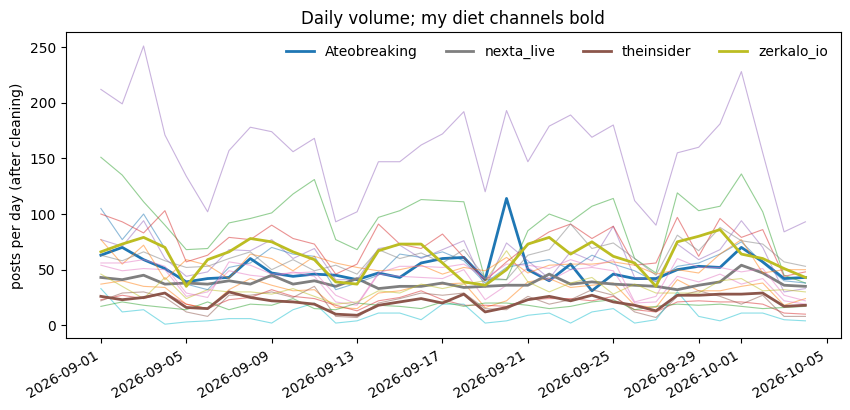
\includegraphics[width=0.82\textwidth]{figures/fig_daily_volume.png}
\caption{Posts per day per channel after cleaning; my four channels are drawn with thick lines. Volumes differ by more than ten times between channels (TASS publishes about 160 posts a day, Pul Pervogo about 10). If channels were pooled post by post, TASS alone would outweigh most of the basket, so every channel average in this report gives each channel equal weight. My four channels publish at a similar, moderate rate; the spike in Ateo Breaking around 20 September coincides with the Russian parliamentary elections and the large drone attacks on Moscow that weekend.}
\label{fig:volume}
\end{figure}

% ------------------------------------------------------------------ 3
\section{Pipeline}
\label{sec:pipeline}

Figure~\ref{fig:pipeline} shows the structure of the analysis. All branches start from the same cleaned table of posts. The classifiers learn what my feed's posts look like word by word. The topic model and the place extraction describe each channel as a probability distribution over subjects or regions, which the echo score then compares. The framing branch counts how the same events are named. The codebook branch checks the topic results against categories I defined myself. Each branch follows the same steps: raw data, preprocessing, a feature matrix, a model fitted on training data, predictions, and an evaluation metric.

\begin{figure}[H]
\centering
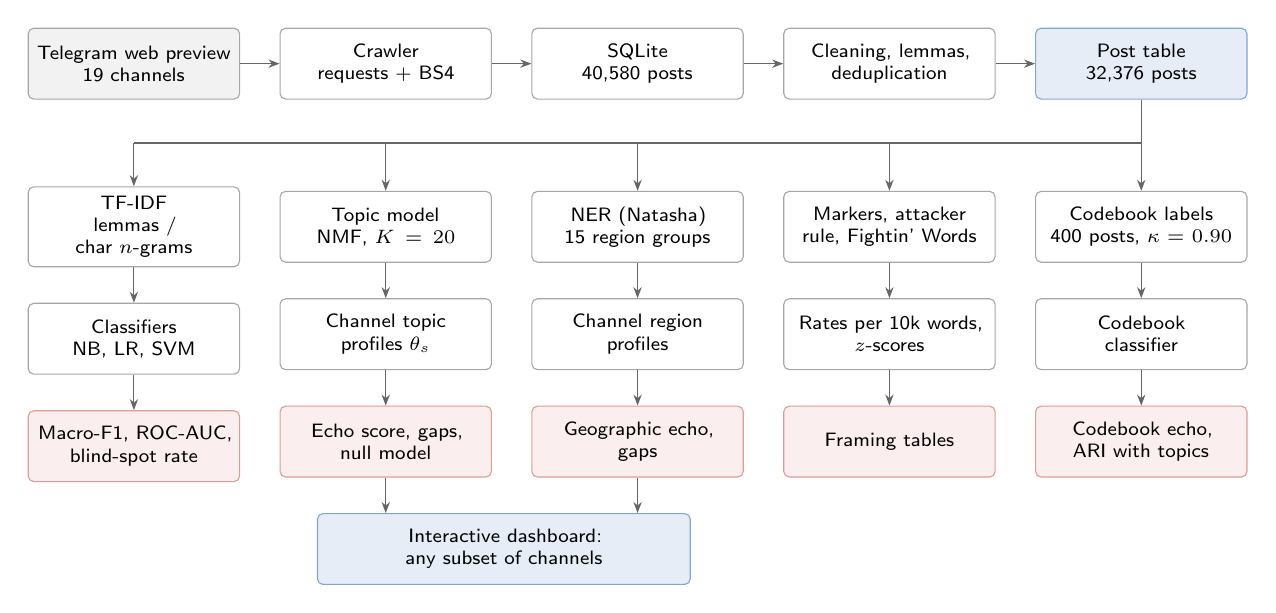
\begin{tikzpicture}[
  node distance=0.45cm and 0.5cm,
  box/.style={draw=black!35,rounded corners=2pt,fill=white,align=center,font=\sffamily\scriptsize,minimum height=0.9cm,text width=2.45cm},
  src/.style={box,fill=black!5},
  data/.style={box,fill=accent!12,draw=accent!60},
  res/.style={box,fill=under!8,draw=under!50},
  arr/.style={-{Stealth[length=4pt]},black!60}]
\node[src] (tg) {Telegram web preview\\ 19 channels};
\node[box,right=of tg] (crawl) {Crawler\\ requests + BS4};
\node[box,right=of crawl] (db) {SQLite\\ 40,580 posts};
\node[box,right=of db] (prep) {Cleaning, lemmas,\\ deduplication};
\node[data,right=of prep] (tab) {Post table\\ 32,376 posts};
\draw[arr] (tg)--(crawl); \draw[arr] (crawl)--(db); \draw[arr] (db)--(prep); \draw[arr] (prep)--(tab);

\node[box,below=1.1cm of tg] (f1) {TF-IDF\\ lemmas / char $n$-grams};
\node[box,right=of f1] (f2) {Topic model\\ NMF, $K=20$};
\node[box,right=of f2] (f3) {NER (Natasha)\\ 15 region groups};
\node[box,right=of f3] (f4) {Markers, attacker\\ rule, Fightin' Words};
\node[box,right=of f4] (f5) {Codebook labels\\ 400 posts, $\kappa=0.90$};

\node[box,below=of f1] (m1) {Classifiers\\ NB, LR, SVM};
\node[box,below=of f2] (m2) {Channel topic\\ profiles $\theta_s$};
\node[box,below=of f3] (m3) {Channel region\\ profiles};
\node[box,below=of f4] (m4) {Rates per 10k words,\\ $z$-scores};
\node[box,below=of f5] (m5) {Codebook\\ classifier};

\node[res,below=of m1] (o1) {Macro-F1, ROC-AUC,\\ blind-spot rate};
\node[res,below=of m2] (o2) {Echo score, gaps,\\ null model};
\node[res,below=of m3] (o3) {Geographic echo,\\ gaps};
\node[res,below=of m4] (o4) {Framing tables};
\node[res,below=of m5] (o5) {Codebook echo,\\ ARI with topics};
\node[data,below=of o2,xshift=1.5cm,text width=4.5cm] (sel) {Interactive dashboard: any subset of channels};

\foreach \a/\b in {f1/m1,m1/o1,f2/m2,m2/o2,f3/m3,m3/o3,f4/m4,m4/o4,f5/m5,m5/o5} \draw[arr] (\a)--(\b);
\path (tab.south) ++(0,-0.55) coordinate (busy);
\draw[black!60] (tab.south) -- (busy);
\draw[black!60] (f1.north |- busy) -- (f5.north |- busy);
\foreach \n in {f1,f2,f3,f4,f5} \draw[arr] (\n.north |- busy) -- (\n.north);
\draw[arr] (o2.south)--(sel.north -| o2.south);
\draw[arr] (o3.south)--(sel.north -| o3.south);
\end{tikzpicture}
\caption{Pipeline. Grey: data source; blue: shared data and the dashboard; red: evaluation outputs. All five analysis branches use the same cleaned post table, so their results can be compared post by post.}
\label{fig:pipeline}
\end{figure}

% ------------------------------------------------------------------ 4
\section{Methods}
\label{sec:methods}

\subsection{Features: TF-IDF}
Each post is represented as a TF-IDF vector over lemmas. A term $t$ in document $d$ receives the weight
\begin{equation}
\mathrm{tfidf}(t,d) = \big(1+\log \mathrm{tf}(t,d)\big)\cdot\left(\log\frac{1+N}{1+\mathrm{df}(t)}+1\right),
\end{equation}
where $\mathrm{tf}(t,d)$ is the number of times $t$ occurs in $d$, $N$ is the number of training posts and $\mathrm{df}(t)$ is the number of posts that contain $t$; each vector is then normalised to unit length. The logarithm on term frequency (``sublinear tf'') keeps a word repeated five times in a long post from dominating the vector, and the inverse document frequency gives less weight to words that appear in most posts. Terms must appear in at least 5 posts, because rarer words cannot be estimated reliably, and in at most half of all posts, because near-universal words carry no information. The vectoriser is fitted on training posts only, so no vocabulary statistic is taken from the test set.

I chose TF-IDF because it is the standard input for linear text classifiers, each model coefficient corresponds to one word and can be read directly, and with 32,000 short documents it is better suited than general-purpose sentence embeddings, which would blur the outlet-specific vocabulary this project measures. As a comparison, character $n$-grams (sequences of 2--5 characters within word boundaries, computed on cleaned but not lemmatised text) capture word endings and spelling directly.

\subsection{Classifiers: can a model tell my feed from the basket?}
The label is $y=1$ if a post comes from one of my four channels and $y=0$ otherwise. Only 19\% of posts are positive, so the class imbalance has to be handled in every model and metric below.

\paragraph{Majority-class baseline} Always predicts ``basket''. It reaches an accuracy of 0.807 without using the text at all, which is why accuracy alone is a poor metric here. Its macro-F1 of 0.446 is the reference that the other models have to exceed.

\paragraph{Multinomial Naive Bayes} A generative model: it models how each class produces words and then applies Bayes' rule,
\begin{equation}
P(y \mid \mathbf{x}) \propto P(y)\prod_{t} P(t \mid y)^{x_t}, \qquad P(t\mid y) = \frac{n_{t,y}+\alpha}{\sum_{t'} n_{t',y} + \alpha |V|},
\end{equation}
where $n_{t,y}$ is the count of term $t$ in class $y$, $|V|$ is the vocabulary size and $\alpha$ is a smoothing constant tuned by cross-validation. It assumes that words are independent given the class, which is not true for text, but it needs little data and is the standard baseline for document classification.

\paragraph{Complement Naive Bayes} Estimates each class's word weights from the documents of the \emph{other} class (Rennie et al., 2003). For the minority class, the complement is the large majority class, so the estimates are less noisy and the model is less affected by class imbalance than multinomial Naive Bayes.

\paragraph{Logistic regression (main model)} A discriminative model of $P(y\mid\mathbf{x})$:
\begin{equation}
P(y=1\mid\mathbf{x}) = \sigma(\mathbf{w}^\top\mathbf{x}+b), \qquad
\min_{\mathbf{w},b}\; \frac{1}{2C}\lVert\mathbf{w}\rVert^2 - \sum_i c_{y_i}\Big[y_i\log \hat p_i + (1-y_i)\log(1-\hat p_i)\Big],
\end{equation}
with class weights $c_y = N/(2N_y)$, so that both classes contribute equally to the loss, and the regularisation strength $C$ chosen from $\{0.3, 1, 3, 10\}$ by three-fold cross-validation on macro-F1 within the training set. I use logistic regression as the main model because it does not assume independent words, it handles correlated features, and its coefficients show which words move a post toward my feed.

\paragraph{Linear support vector machine} Finds the separating hyperplane with the largest margin in TF-IDF space (hinge loss instead of log loss). It is often the strongest linear text classifier. Platt scaling converts its scores into probabilities so that it can be compared with the other models on ROC-AUC.

\paragraph{Evaluation design}
\begin{itemize}
\item \textbf{Temporal split.} Posts before 26 September are used for training and later posts for testing. News stories run over several days, so a random split would place posts about the same event in both sets and reward memorising events. The random split is reported for comparison.
\item \textbf{Leave one channel out.} Each channel is held out in turn and scored by a model trained on the other 18. This tests whether the model learned something general about my feed or only recognises the four specific channels.
\item \textbf{Metrics.} Macro-F1 averages the F1 score over both classes, so the minority class counts equally. ROC-AUC measures how well the model ranks posts, independently of any threshold: it is the probability that a random post from my feed receives a higher score than a random basket post.
\item \textbf{Threshold tuning.} Class weights inflate the predicted probabilities for the minority class, so the default threshold of 0.5 does not maximise macro-F1. The threshold is chosen on a validation set (the last 20\% of the training period) and then applied once to the test set.
\end{itemize}

\subsection{Topic models: what subjects does each channel cover?}
\paragraph{Latent Dirichlet Allocation (LDA)} A generative model in which each post is a mixture of $K$ topics and each topic is a probability distribution over words (Blei et al., 2003):
\begin{equation}
\theta_d \sim \mathrm{Dir}(\alpha), \qquad z_{dn} \sim \mathrm{Cat}(\theta_d), \qquad w_{dn} \sim \mathrm{Cat}(\beta_{z_{dn}}).
\end{equation}
Here $\theta_d$ is post $d$'s topic mix, $z_{dn}$ is the topic of its $n$-th word and $\beta_k$ is topic $k$'s word distribution. The posterior over $\theta$ and $\beta$ cannot be computed exactly and is approximated by online variational Bayes.

\paragraph{Non-negative matrix factorisation (NMF)} Factorises the post--term TF-IDF matrix $X$ into two non-negative matrices (Lee \& Seung, 1999):
\begin{equation}
\min_{W \geq 0,\, H \geq 0} \; \lVert X - WH \rVert_F^2 .
\end{equation}
The rows of $H$ are topics; row $d$ of $W$, normalised to sum to one, is post $d$'s topic mix $\theta_d$. NMF has no probabilistic model, but the non-negativity constraint produces additive, parts-based topics, and it works directly on TF-IDF weights, which suits short texts with low word counts.

\paragraph{News stoplist} Before topic modelling, reporting verbs (сообщить ``to report'', заявить ``to state''), time words (год ``year'', день ``day'') and format words (видео ``video'', читать ``to read'', канал ``channel'') are removed, because they appear in posts on every subject and would otherwise form ``topics'' of their own (Schofield et al., 2017). The classifier keeps these words, because they are part of an outlet's style.

\paragraph{Model selection} Held-out perplexity increased with $K$ and therefore always selected the smallest number of topics tested; perplexity is known to be a weak guide to interpretable topics. Instead, each candidate (LDA and NMF, $K\in\{8,12,16,20,25,30\}$) is scored on two criteria:
\begin{itemize}
\item \textbf{Coherence}: the mean normalised pointwise mutual information over all pairs of a topic's ten top words, where $P(w)$ is the share of posts containing $w$ (Bouma, 2009; Röder et al., 2015):
\begin{equation}
\mathrm{NPMI}(w_i, w_j) = \frac{\log \dfrac{P(w_i, w_j)}{P(w_i)\,P(w_j)}}{-\log P(w_i, w_j)} \in [-1, 1].
\end{equation}
NPMI is $+1$ when two words always occur together, 0 when they occur independently and $-1$ when they never occur together. A coherent topic consists of words that appear in the same posts.
\item \textbf{Stability}: the adjusted Rand index (ARI; Hubert \& Arabie, 1985) between the post-to-topic assignments of three runs with different random seeds. ARI is corrected for chance: 0 means no more agreement than random labels and 1 means identical partitions. If a model is unstable, part of what its topics show is the random initialisation rather than the data.
\end{itemize}
The selection rule was fixed before I read any topics: among candidates with ARI $\geq 0.5$, choose the one with the highest coherence. A channel's topic profile $\theta_s$ is the mean topic mix of its posts.

\subsection{Named-entity recognition: which places does each channel cover?}
Natasha's \texttt{NewsNERTagger}, a neural sequence tagger trained on Russian news, marks spans of text that name locations. Each span is lemmatised with pymorphy3, for example \ru{Харьковскую область}{Kharkiv region, in the accusative case} becomes «харьковский область» (the dictionary forms of both words), and mapped to one of 15 region groups. Crimea, the Donbas (the occupied parts of the Donetsk and Luhansk regions) and the Black Sea are kept as separate groups rather than assigned to a country. Two names that the tagger marks as locations but that are not places in this sense, «запад» (``the West'', a political bloc) and «СССР» (the USSR), are excluded; the mapping covers 74\% of the remaining location mentions. Russia annexed Crimea in 2014 and claims the Donbas, while most other states recognise both as part of Ukraine; Russian state media therefore report events there as domestic news and Ukrainian media as news from occupied territory. Assigning them to either country would build one side's position into the measurement, and they are also distinct news areas in their own right. A post counts once for every region group it mentions, and a channel's region profile is the share of its location mentions in each group. 26,043 of the 32,376 posts mention at least one place.

\subsection{Codebook labels: categories defined by hand}
\label{sec:codebook-method}
The topic model determines the categories itself. As a check that does not depend on it, I wrote a codebook of 14 categories (Table~\ref{tab:codebook}) with written rules for borderline cases before any posts were classified.

\paragraph{Sample} 400 posts, stratified by NMF topic and by my feed versus the basket so that every topic and both groups are represented. The posts were shuffled and shown \emph{without the channel name}, so that the source could not influence the label.

\paragraph{Two annotators} I labelled 200 of the posts by hand. A large language model (Claude, Anthropic) labelled all 400 using the same codebook and rules, without access to my labels. Agreement on the 200 shared posts is measured with Cohen's kappa, which corrects the observed agreement $p_o$ for the agreement $p_e$ expected by chance given each annotator's label frequencies $\hat\pi_c$:
\begin{equation}
\kappa = \frac{p_o - p_e}{1 - p_e}, \qquad p_e = \sum_{c} \hat\pi^{(1)}_c\,\hat\pi^{(2)}_c .
\end{equation}
The rule, set in advance, was to train on the LLM's 400 labels only if $\kappa \geq 0.6$ (``substantial'' agreement), and otherwise on my 200.

\paragraph{From the sample to the corpus} A logistic regression on TF-IDF features learns the codebook from the labelled posts (five-fold stratified cross-validation; categories with fewer than five examples are merged into ``Other'') and then labels all 32,376 posts. The resulting labels are compared with the NMF topics using the adjusted Rand index, and the echo score and null model of Section~\ref{sec:metrics} are recomputed with codebook categories in place of topics.

\begin{table}[H]
\centering
\small
\caption{The codebook.}
\label{tab:codebook}
\begin{tabular}{rl@{\hspace{2em}}rl}
\toprule
1 & War: strikes and casualties & 8 & Belarus: state agenda \\
2 & War: front line and military operations & 9 & Belarus: repression and political prisoners \\
3 & War: diplomacy and international reaction & 10 & Belarus: society and other \\
4 & Ukraine: domestic politics and society & 11 & USA, EU and international politics \\
5 & Russia: politics, government and elections & 12 & Accidents, crime and incidents (not war) \\
6 & Russia: repression, courts and censorship & 13 & Culture, sport and lifestyle \\
7 & Russia: economy and business & 14 & Other \\
\bottomrule
\end{tabular}
\end{table}

\subsection{New metrics}
\label{sec:metrics}
\paragraph{Echo score} The basket profile $p_R$ is the unweighted mean of all 19 channel profiles $\theta_s$ (topic mixes, or region shares in the geographic version). My feed's profile $q_D$ weights my four channels by reading share $w_s$:
\begin{equation}
p_R = \frac{1}{|R|}\sum_{s\in R}\theta_s, \qquad q_D = \sum_{s\in D} w_s\,\theta_s, \qquad \Echo(D) = \JSD(q_D \,\|\, p_R),
\end{equation}
\begin{equation}
\JSD(q\,\|\,p) = \tfrac{1}{2}\,\KL(q\,\|\,m) + \tfrac{1}{2}\,\KL(p\,\|\,m), \qquad m = \tfrac{1}{2}(q+p), \qquad \KL(q\,\|\,m)=\sum_k q_k\log_2\frac{q_k}{m_k}.
\end{equation}
I use the Jensen--Shannon divergence (Lin, 1991) rather than the KL divergence because it is symmetric, it remains finite when a topic is absent from one side, and in base 2 it lies between 0 (identical distributions) and 1 (no overlap).

\paragraph{Coverage gap} The log ratio per topic (or per region) shows which topics drive the score:
\begin{equation}
g_k = \log\frac{q_{D,k}}{p_{R,k}} .
\end{equation}
A value of $g_k=-0.69$ means that my feed gives topic $k$ half the basket's share; $g_k=+0.69$ means twice the share.

\paragraph{Null model} An echo score on its own has no natural scale. With 19 channels there are $\binom{19}{4}=3{,}876$ possible four-channel feeds, so I score every one of them (with equal weights within a feed) and report the percentile of my feed among them. This is an exact reference distribution rather than a random sample.

\paragraph{Uncertainty} A bootstrap resamples posts with replacement within each channel, recomputes every $\theta_s$ and the echo score, and repeats this 300 times; the 2.5th and 97.5th percentiles form the 95\% interval. A sensitivity check drops each basket channel in turn and recomputes $p_R$, to show how much the result depends on my choice of basket.

\paragraph{Blind-spot score} For each basket post $i$, using out-of-fold probabilities from five-fold cross-validation so that no post is scored by a model trained on it:
\begin{equation}
B_i = 1 - \hat{P}(\text{my feed} \mid \mathbf{x}_i), \qquad
\mathrm{BSR}_k(\tau) = \frac{1}{N_k}\sum_{i\in k}\mathbb{1}\!\left[\hat{P}(\text{my feed}\mid \mathbf{x}_i) < \tau\right].
\end{equation}
$\mathrm{BSR}_k$ is the share of topic $k$'s basket posts that the classifier considers very unlike my feed. It is computed for $\tau\in\{0.1,0.2,0.3\}$ to check that the ranking of topics does not depend on the threshold.

\subsection{Framing}
\paragraph{Marker words} Counts per 10,000 words of words that indicate a stance or a source. These include the name of the war (\ru{война}{war}, \ru{СВО}{``special military operation''}, \ru{вторжение}{invasion}); the abbreviation for the Ukrainian armed forces (\ru{ВСУ}{Russian-language abbreviation} and \ru{ЗСУ}{Ukrainian-language abbreviation}); \ru{киевский режим}{``Kyiv regime''}; the two spellings of ``Belarusian'', «белорусский» (official and Russian standard) and «беларусский» (used by the Belarusian opposition); \ru{политзаключенный}{political prisoner}; \ru{иноагент}{``foreign agent''}; attribution and distancing words (\ru{по словам}{according to}, \ru{якобы}{allegedly}, \ru{так называемый}{so-called}); and named sources (the Russian Ministry of Defence, the Ukrainian military, the Institute for the Study of War).

\paragraph{Attacker rule} Within the six strike-related topics (6,286 posts), a word-pattern rule records whether the Russian or the Ukrainian side is named as the attacker. It looks for a side word (\ru{российский}{Russian}, \ru{Россия}{Russia}, \ru{ВС РФ}{Armed Forces of the Russian Federation}; \ru{украинский}{Ukrainian}, \ru{ВСУ}{Armed Forces of Ukraine}) within one word of an attack word (\ru{удар}{strike}, \ru{атака}{attack}, \ru{обстрел}{shelling}, \ru{дрон}{drone}, \ru{ракета}{missile}, \ru{БПЛА}{unmanned aerial vehicle}). Matches in which the side is the target, such as \ru{удар по российскому НПЗ}{a strike on a Russian oil refinery}, or a place, such as \ru{сбили над регионами России}{shot down over Russian regions}, are excluded. I checked the rule by reading a random sample of 30 matches per side.

\paragraph{Fightin' Words} To find the words most typical of one group of outlets compared with another, a raw log-odds ratio is unreliable, because rare words get extreme ratios from very small counts. Monroe, Colaresi and Quinn (2008) shrink each word toward its overall frequency with an informative Dirichlet prior ($\alpha_w$ proportional to the word's frequency in the corpus, $\alpha_0=500$ pseudo-counts) and divide by an approximate standard error:
\begin{equation}
\delta_w = \log \frac{y_w^a + \alpha_w}{n^a + \alpha_0 - y_w^a - \alpha_w} - \log \frac{y_w^b + \alpha_w}{n^b + \alpha_0 - y_w^b - \alpha_w}, \qquad
z_w = \frac{\delta_w}{\sqrt{\dfrac{1}{y_w^a + \alpha_w} + \dfrac{1}{y_w^b + \alpha_w}}},
\end{equation}
where $y_w^a$ is the count of word $w$ in group $a$ and $n^a$ is the total word count of group $a$. The variance term follows from the delta method: the variance of the logarithm of a Poisson count $y$ is approximately $1/y$. Words with $|z|>1.96$ are distinctive at about the 5\% level. A first run with $\alpha_0=10{,}000$ shrank almost every word to zero; with 500, rare words are stabilised while frequent words stay close to their observed rates.

% ------------------------------------------------------------------ 5
\section{Results}
\label{sec:results}

\subsection{Classifiers}
\label{sec:res-classifier}
Each row of Table~\ref{tab:models} changes one setting relative to the baseline (logistic regression, lemmas, single words, temporal split, cleaned text).

\begin{table}[H]
\centering
\small
\caption{Classifier comparison on the temporal test set (81\% of test posts come from the basket).}
\label{tab:models}
\begin{tabular}{lccc}
\toprule
Condition & Accuracy & Macro-F1 & ROC-AUC \\
\midrule
Dummy (always ``basket'') & 0.807 & 0.446 & 0.500 \\
Multinomial Naive Bayes & 0.827 & 0.586 & 0.791 \\
Complement Naive Bayes & 0.762 & 0.672 & 0.791 \\
Linear SVM (Platt-scaled) & 0.835 & 0.639 & 0.818 \\
\textbf{Logistic regression (baseline)} & \textbf{0.780} & \textbf{0.694} & \textbf{0.821} \\
Logistic regression, threshold tuned to 0.63 & 0.822 & 0.705 & 0.821 \\
Logistic regression, single words + word pairs & 0.813 & 0.718 & 0.838 \\
Logistic regression, character 2--5-grams & 0.837 & \textbf{0.769} & \textbf{0.896} \\
\midrule
Logistic regression, random split & 0.804 & 0.715 & 0.841 \\
Logistic regression, raw text (signatures and names kept) & 0.877 & 0.814 & 0.935 \\
Logistic regression, leave one channel out & --- & --- & 0.503 \\
\bottomrule
\end{tabular}
\end{table}

\begin{figure}[H]
\centering
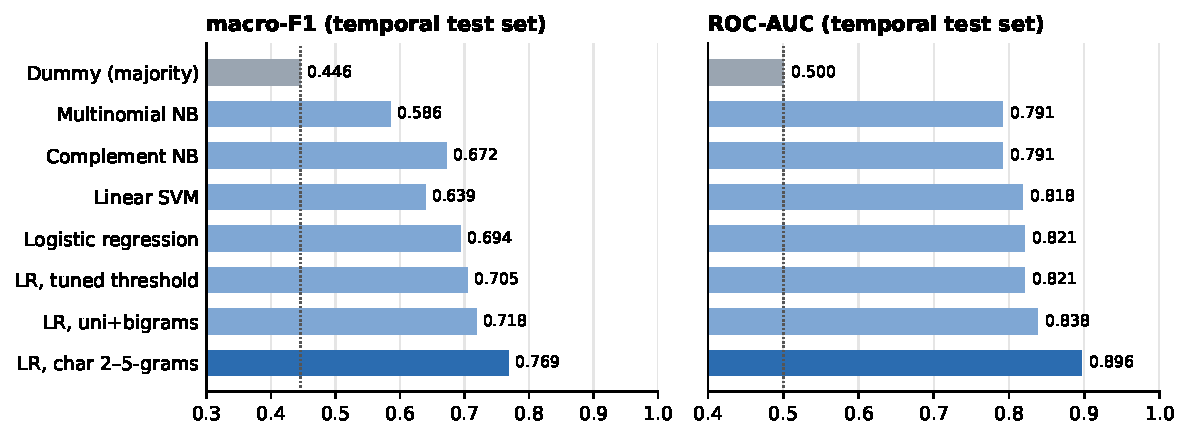
\includegraphics[width=\textwidth]{figures/fig_models.pdf}
\caption{Macro-F1 (left) and ROC-AUC (right) of every classifier on the temporal test set; the dotted lines mark the majority-class baseline (macro-F1 0.446) and chance (ROC-AUC 0.5). All models rank posts much better than chance, but they differ more on macro-F1 than on ROC-AUC: the two Naive Bayes models have the same ROC-AUC (0.791) but different macro-F1 (0.586 and 0.672), because they rank posts similarly but place the decision threshold differently. Character $n$-grams (dark blue) are best on both measures.}
\label{fig:models}
\end{figure}

\paragraph{Naive Bayes ranks posts well but classifies them poorly} Multinomial Naive Bayes reaches a ROC-AUC of 0.79 but a macro-F1 of only 0.586, because it predicts ``my feed'' for just 16\% of my feed's test posts (Figure~\ref{fig:confusion}b). The independence assumption multiplies hundreds of word likelihoods as if each were separate evidence, which pushes the posterior probabilities toward 0 or 1, and the 81\% prior then assigns most posts to the basket. The \emph{ranking} of posts remains informative, and that is what ROC-AUC measures. Complement Naive Bayes, whose estimates for the minority class come from the large complement class, raises macro-F1 to 0.672.

\paragraph{Logistic regression and the default threshold} At the default threshold of 0.5, logistic regression has lower accuracy than the dummy (0.780 compared with 0.807) but a much higher macro-F1. Class weighting trains the model as if the two classes were the same size, so its probabilities for ``my feed'' are too high and a threshold of 0.5 produces many false positives (19\% of basket posts). A threshold of 0.63, chosen on the validation set, reduces false positives to 10\% and raises accuracy to 0.822 and macro-F1 to 0.705, at the cost of recall on my feed (0.64 to 0.50). ROC-AUC is unchanged, because moving the threshold does not change the ranking.

\begin{figure}[H]
\centering
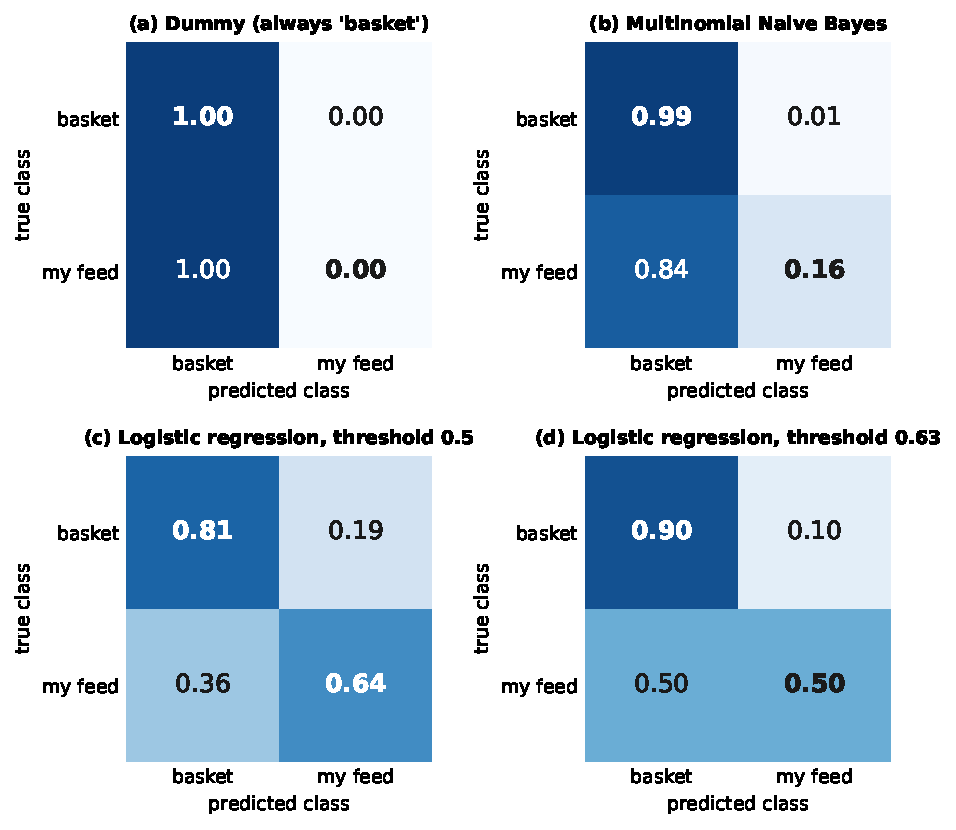
\includegraphics[width=0.72\textwidth]{figures/fig_confusion.pdf}
\caption{Normalised confusion matrices on the temporal test set. Rows are the true class and sum to 1; the diagonal (bold) shows correct predictions. (a) The dummy assigns every post to the basket, so its recall on my feed is 0. (b) Multinomial Naive Bayes is almost the same: it finds only 16\% of my feed's posts. (c) Logistic regression at threshold 0.5 finds 64\% of my feed's posts but also marks 19\% of basket posts as mine. (d) At the tuned threshold of 0.63, false positives fall to 10\% and recall on my feed falls to 50\%. Panels (c) and (d) show the same model with different thresholds, which illustrates the trade-off between precision and recall.}
\label{fig:confusion}
\end{figure}

\paragraph{Character n-grams perform best} Character 2--5-grams reach a macro-F1 of 0.769 and a ROC-AUC of 0.896. Russian expresses much of its grammar through word endings, and character $n$-grams see endings, spelling variants and morphology that lemmatisation removes on purpose. Part of the improvement is therefore stylistic: «беларусский» and «белорусский» (two spellings of ``Belarusian'') differ in one letter, and a three-character window detects the difference. This supports the interpretation in Section~\ref{sec:res-agenda} that my feed is recognised by style rather than by content.

\paragraph{Channel signatures} Keeping channel signatures and outlet names in the text raises ROC-AUC from 0.82 to 0.94. A classifier trained on raw text would largely be recognising signatures, a form of data leakage comparable to an image classifier that learns camera resolution instead of content. This is the reason for the cleaning step in Section~\ref{sec:data}.

\paragraph{Temporal and random splits} The two splits give similar results (ROC-AUC 0.821 and 0.841), so the model does not rely on recognising specific news events that appear in both the training and the test data.

\paragraph{Errors by channel} Figure~\ref{fig:perchannel} breaks the predictions down by channel. At the tuned threshold the classifier recognises 70\% of Zerkalo's test posts, 49\% of NEXTA's and 40\% of Ateo's, but only 21\% of The Insider's; The Insider publishes long investigative posts that are closer in style to the exile media in the basket than to the rest of my feed. The basket channels most often mistaken for my feed are UNIAN (21\%), which uses similar war vocabulary, Meduza (19\%), which shares the exile style, and BelTA (16\%), which covers the same Belarusian subjects. The pro-war blog Rybar is almost never mistaken for my feed (0.6\%). The words with the largest coefficients toward my feed are «беларусский» (Belarusian, opposition spelling), \ru{Тихановский}{Tsikhanouski, a surname}, \ru{политзаключенный}{political prisoner}, \ru{диктатор}{dictator} and \ru{Вясна}{Viasna, a Belarusian human-rights centre}; toward the basket, the reporting verbs \ru{сообщить}{to report} and \ru{отметить}{to note}, \ru{ВСУ}{Armed Forces of Ukraine} and «белорусский» (Belarusian, official spelling).

\begin{figure}[H]
\centering
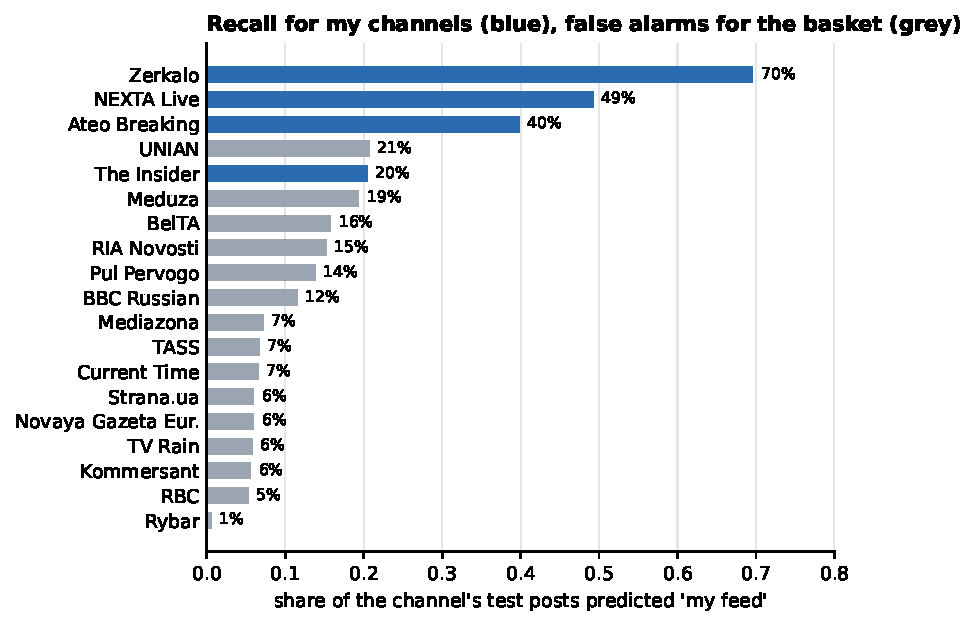
\includegraphics[width=0.66\textwidth]{figures/fig_per_channel.pdf}
\caption{Share of each channel's test posts predicted as ``my feed'' at the tuned threshold. For my four channels (blue) this is recall, so a longer bar is better; for basket channels (grey) it is the false-positive rate, so a shorter bar is better. Zerkalo is recognised most often and The Insider least. Among basket channels, false positives are concentrated in outlets that share either my feed's subjects (UNIAN, BelTA) or its style (Meduza), while state media and the pro-war blog are rarely confused with it.}
\label{fig:perchannel}
\end{figure}

\subsection{Agenda or style?}
\label{sec:res-agenda}
Within the corpus the classifier performs well; on a channel it has not seen, it performs at chance (ROC-AUC 0.503). The label is \emph{channel membership}, so when all four of my channels are in the training data the model can learn each channel's habits, but when one channel is held out, what the model learned from the other three does not transfer to it. To test whether the model learns anything about subject matter, the same logistic regression was trained on each post's 20-topic mix instead of its words (Table~\ref{tab:agenda}).

\begin{table}[H]
\centering
\small
\caption{Words versus topic mixes as features.}
\label{tab:agenda}
\begin{tabular}{lcc}
\toprule
Features & ROC-AUC, temporal split & ROC-AUC, leave one channel out \\
\midrule
TF-IDF over lemmas & 0.821 & 0.503 \\
Topic mix (NMF, $K=20$) & 0.606 & 0.370 \\
\bottomrule
\end{tabular}
\end{table}

Topic features perform worse in both settings. A value \emph{below} 0.5 on held-out channels means that when one of my channels is left out, a model trained on the other three ranks its posts systematically below the basket. My four channels differ from each other in topics about as much as they differ from the basket, so a topic profile learned from three of them does not fit the fourth. There is no shared agenda for the model to learn; my feed is recognisable by how it is written, which agrees with the low topic echo score reported below.

\subsection{Choosing the topic model}
NMF produces topics about twice as coherent as LDA's and much more stable across seeds (Figure~\ref{fig:topicsel}, Table~\ref{tab:topicsel}). LDA's topics changed with the random seed at every $K$ (ARI around 0.2). This is expected from how LDA is estimated: the variational objective is non-convex with many local optima, and short posts (a few dozen lemmas each) give so few word counts per document that the data barely constrain each post's topic mix, so the starting point determines much of the result. NMF with an SVD-based initialisation (NNDSVD) starts from a deterministic point derived from the data and converges to similar solutions. The selection rule chose \textbf{NMF with 20 topics} (coherence 0.337, stability 0.59). No two of its topics overlap: no pair of topic-word vectors has a cosine similarity above 0.4.

\begin{figure}[H]
\centering
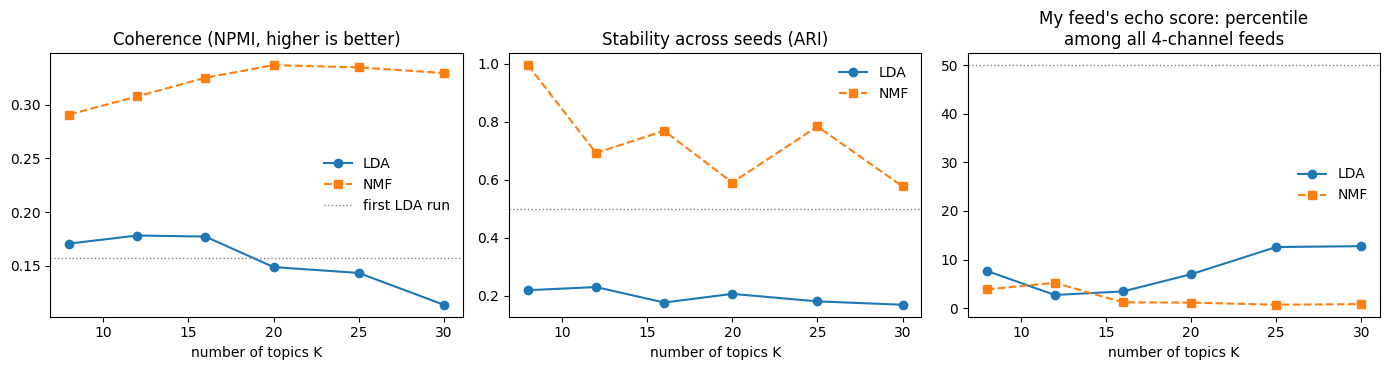
\includegraphics[width=\textwidth]{figures/fig_topic_model_selection.png}
\caption{Topic-model selection for LDA (blue) and NMF (orange) at $K=8$ to 30. Left: coherence (higher is better); NMF is above LDA at every $K$ and peaks at $K=20$; the dotted line is my first LDA run ($K=8$, no news stoplist, coherence 0.158). Middle: stability across three seeds; the dotted line is the 0.5 threshold, which only NMF passes. Right: my feed's echo-score percentile among all four-channel feeds. It stays below 13\% under every candidate model, so the main finding does not depend on which topic model is chosen.}
\label{fig:topicsel}
\end{figure}

\begin{table}[H]
\centering
\small
\caption{Topic-model candidates, $K=8$--30.}
\label{tab:topicsel}
\begin{tabular}{lccc}
\toprule
Method & Coherence (NPMI) & Stability (ARI) & Echo percentile \\
\midrule
LDA, first run ($K=8$, chosen by perplexity) & 0.158 & --- & 31\% \\
LDA, news stoplist & 0.114--0.178 & 0.17--0.23 & 2.7--12.8\% \\
\textbf{NMF, news stoplist} & \textbf{0.291--0.337} & \textbf{0.58--1.00} & \textbf{0.7--5.2\%} \\
\bottomrule
\end{tabular}
\end{table}

I labelled the 20 topics by hand from their top words and most typical posts. They range from strikes on Ukrainian infrastructure, air-defence reports and front-line territorial claims to the Russian parliamentary (Duma) elections, US--Russia talks, sanctions, oil prices and Belarus's state agenda. Two topics are imperfect: T1 combines strike casualties with road accidents, and T11 is a single story (a fight between pilots on a Flydubai flight).

\subsection{How broad is my feed?}
\textbf{By topic, my feed is closer to the basket than almost any other four-channel feed.} Its echo score is 0.0038 with reading weights (95\% bootstrap interval 0.0032--0.0046) and 0.0034 with equal weights, which is lower than 98.2\% of the 3,876 possible four-channel feeds (Figure~\ref{fig:null}). The result holds for every candidate topic model (Figure~\ref{fig:topicsel}, right). Dropping any one basket channel changes the score only within 0.0035--0.0047; the largest changes come from dropping BelTA or Pul Pervogo, the two Belarusian state channels.

\begin{figure}[H]
\centering
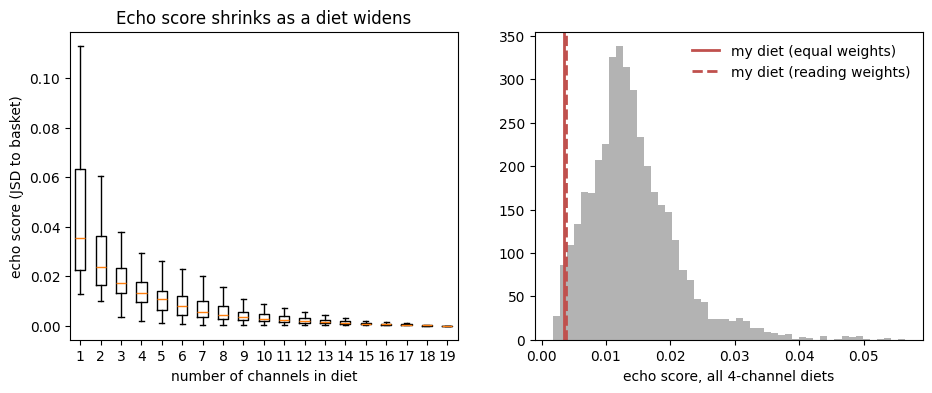
\includegraphics[width=0.92\textwidth]{figures/fig_null_model.png}
\caption{Null model. Left: echo scores of all possible feeds, grouped by number of channels. Each box spans the middle 50\% of feeds of that size (first to third quartile), the orange line is the median, and the whiskers extend to the most extreme feed within 1.5 times the box height; feeds beyond the whiskers are not drawn. Single channels range from about 0.01 to 0.11, and both the median and the spread shrink as feeds grow, until a feed of all 19 channels equals the basket (score 0). Right: histogram of all 3,876 four-channel feeds. Most score between 0.005 and 0.025; my feed (solid line, equal weights; dashed line, reading weights) is at the far left of the distribution, among the 2\% of feeds closest to the basket.}
\label{fig:null}
\end{figure}

\paragraph{Why the score is low} The Jensen--Shannon divergence is convex in its first argument, so the divergence of a mixture is at most the weighted average of the divergences of its parts:
\begin{equation}
\JSD\Big(\sum_{s\in D} w_s\theta_s \,\Big\|\, p_R\Big) \;\leq\; \sum_{s\in D} w_s\, \JSD(\theta_s\,\|\,p_R).
\end{equation}
The mixture's divergence is much smaller than this upper bound when the parts deviate from $p_R$ in \emph{different} directions, because their deviations cancel in the average. Each of my four channels is far from the basket on its own (a Belarusian outlet, an investigative outlet and two breaking-news feeds), but they deviate in different directions, so their mixture is close to the basket average. Convexity also explains the left panel of Figure~\ref{fig:null}: as a feed includes more channels, its mixture moves toward $p_R$ and the spread of scores decreases. The bootstrap interval is narrow because each channel profile is an average over hundreds or thousands of posts, so its sampling error, which scales with $1/\sqrt{n}$, is small.

\subsection{Sensitivity to reading weights}
\label{sec:weights}
The reading weights are my own estimate, so I drew 2,000 random weightings of my four channels from a flat Dirichlet distribution, in which every combination of weights that sums to one is equally likely, and recomputed the echo score for each (Figure~\ref{fig:weights}, Table~\ref{tab:single}).

\begin{table}[H]
\centering
\small
\caption{Echo score over 2,000 random reading weightings, and the echo score of each of my channels read on its own. ``Percentile'' is the share of all four-channel feeds that are closer to the basket than my feed (lower means broader).}
\label{tab:single}
\begin{tabular}{lcc}
\toprule
 & Topic echo score & Percentile \\
\midrule
My reading weights & 0.0038 & 1.8\% (equal weights) \\
Random weights, median & 0.0078 & 16.2\% \\
Random weights, middle 90\% of draws & 0.0040--0.0213 & 3.2--87.9\% \\
\midrule
The Insider only & 0.0180 & \\
NEXTA Live only & 0.0200 & \\
Ateo Breaking only & 0.0315 & \\
Zerkalo only & 0.0530 & \\
\bottomrule
\end{tabular}
\end{table}

\begin{figure}[H]
\centering
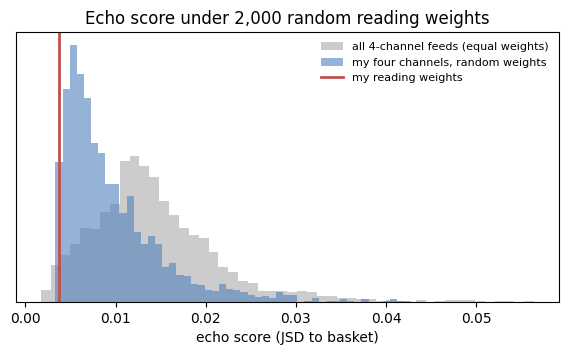
\includegraphics[width=0.7\textwidth]{figures/fig_weight_sensitivity.png}
\caption{Echo score of my four channels under 2,000 random reading weightings (blue), compared with all 3,876 equal-weight four-channel feeds (grey). The red line is my estimated weights. Most random weightings fall to the left of the grey distribution's centre, but a long tail reaches into it: these are weightings in which one channel, usually Zerkalo, takes most of the weight.}
\label{fig:weights}
\end{figure}

The result depends on how evenly I read my channels. With my estimated weights and with equal weights, my feed is among the 2\% of feeds closest to the basket. Across random weightings the median percentile is 16\%, and 80\% of weightings are still closer to the basket than the median four-channel feed. Each channel on its own is much further from the basket (0.018--0.053) than any mixture of them, which is the convexity effect described above: the channels are narrow individually and broad together. Zerkalo, the Belarusian outlet, is the narrowest; a feed that consisted mostly of Zerkalo would be narrower than most four-channel feeds. Which topics are under-covered is more stable than how strongly: on average, 61\% of the three most under-covered topics under my weights are also among the three most under-covered under a random weighting. For places, the median percentile over random weightings is 32\% (middle 90\%: 10--98\%), so the geographic result is more sensitive to the weights than the topic result.

\subsection{What my feed under-covers}
\paragraph{Topics} The gaps are small in absolute terms but consistent (Figure~\ref{fig:topicgap}, Table~\ref{tab:gaps}). My feed under-covers military bulletins from both sides: Russian Ministry of Defence claims about captured villages, air-defence tallies such as \ru{силы ПВО сбили N БПЛА}{air defence shot down N drones}, and local updates on strikes from the mayor of Kyiv. It over-covers US politics, drone attacks as a subject, and the debate between Russia, European countries and NATO.

\begin{figure}[H]
\centering
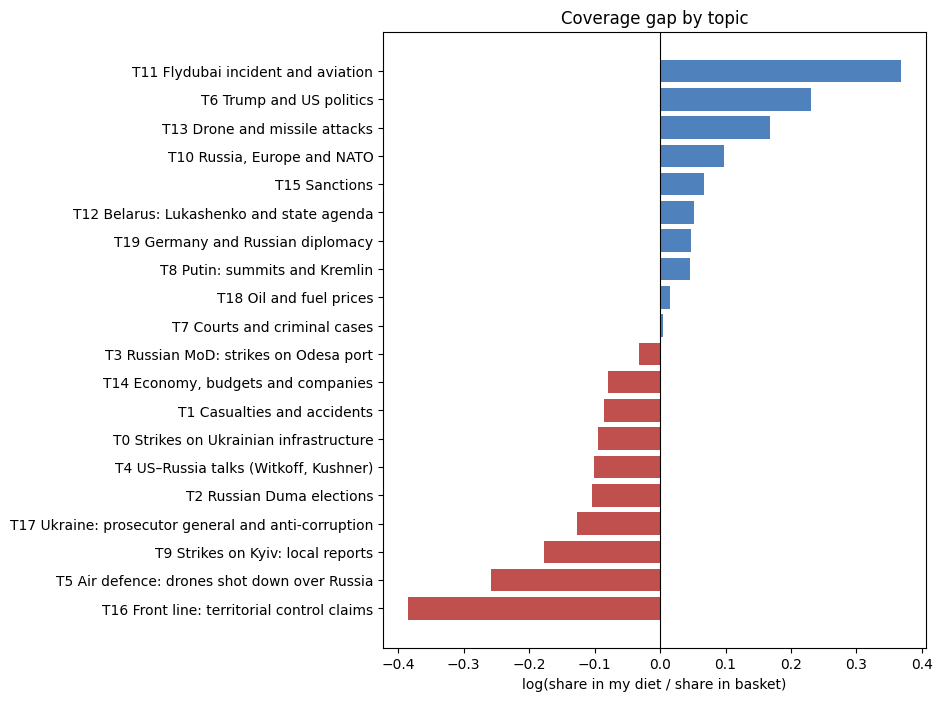
\includegraphics[width=0.72\textwidth]{figures/fig_topic_gaps.png}
\caption{Coverage gap $g_k = \log(q_{D,k}/p_{R,k})$ for each of the 20 topics, sorted from most over-covered (top) to most under-covered (bottom). Blue bars (positive values) are topics that take a larger share of my feed than of the basket; red bars (negative values) are topics my feed covers less. A bar at $-0.39$, as for T16, means my feed gives that topic about 68\% of the basket's share ($e^{-0.39}\approx0.68$). Three of the four most under-covered topics are routine war reporting (front-line claims, air defence, local strike reports); the fourth is Ukrainian domestic politics. The most over-covered include a single event (T11, the Flydubai incident) and US politics.}
\label{fig:topicgap}
\end{figure}

\begin{table}[H]
\centering
\small
\caption{Largest topic gaps and the classifier's blind-spot rate for the same topics. ``My feed'' and ``Basket'' are the topic's share of all posts in each. The gap $g_k$ is negative (shown in red) when my feed covers the topic less than the basket and positive when it covers it more; $-0.39$ corresponds to about two-thirds of the basket's share and $+0.37$ to about one and a half times. The blind-spot rate (BSR) is the share of the topic's basket posts that the classifier considers very unlike my feed ($\hat P < 0.2$); a higher value means the topic's posts are written in a way my feed does not resemble. Topics with negative gaps have high blind-spot rates (0.55--0.71) and topics with positive gaps low ones (about 0.3), so the two measures agree.}
\label{tab:gaps}
\begin{tabular}{lcccc}
\toprule
Topic & My feed & Basket & Gap $g_k$ & BSR ($\tau=0.2$) \\
\midrule
T16 Front line: territorial-control claims & 2.8\% & 4.1\% & \gap{$-0.39$} & 0.69 \\
T5 Air defence: drones shot down over Russia & 1.9\% & 2.4\% & \gap{$-0.26$} & 0.71 \\
T9 Strikes on Kyiv: local reports & 2.9\% & 3.5\% & \gap{$-0.18$} & 0.61 \\
T17 Ukraine: prosecutor general dismissal & 2.5\% & 2.9\% & \gap{$-0.14$} & 0.55 \\
T13 Drone and missile attacks & 6.1\% & 5.2\% & $+0.17$ & 0.33 \\
T6 Trump and US politics & 5.0\% & 4.0\% & $+0.23$ & 0.31 \\
T11 Flydubai incident & 4.8\% & 3.3\% & $+0.37$ & 0.32 \\
\bottomrule
\end{tabular}
\end{table}

The blind-spot rate is computed from the classifier, which works on a different principle from the topic model. It ranks the same topics highest (T3, strikes on the port of Odesa, also reaches 0.71) and the same over-covered topics lowest. One method is unsupervised and works on distributions over topics; the other is supervised and works on individual posts. Because they agree, the identified gaps are unlikely to be an artefact of either method.

\paragraph{What the blind spots look like} For each of the three most under-covered topics, the basket posts that the classifier considers least like my feed are short, formulaic bulletins (translated; $\hat P$ is the predicted probability that the post belongs to my feed):
\begin{itemize}
\item \textbf{T16, front line} (RIA Novosti, 14 September, $\hat P=0.002$): ``Special operation. Situation and main events on 14 September: the Russian army liberated Shirokoye and Shevchenkovo in the area where Ukrainian forces are encircled in the Kharkiv region, and Novoandreyevka in the Zaporizhzhia region, according to the Ministry of Defence summary.''
\item \textbf{T5, air defence} (RIA Novosti, 26 September, $\hat P=0.002$): ``Air defence shot down 1,222 drones of the Ukrainian Armed Forces in one day, the Ministry of Defence said.''
\item \textbf{T9, strikes on Kyiv} (Strana.ua, 29 September, $\hat P=0.001$): ``Explosion in Kyiv. Klitschko reports a hit on a non-residential building in the Podilskyi district. Local public pages are publishing video of the fire.''
\end{itemize}
These are the reports my channels summarise rather than repeat: official military claims in the language of the Russian Ministry of Defence (``liberated'', ``Ukrainian Armed Forces''), and minute-by-minute local updates from Kyiv.

\paragraph{Places} Geography separates my feed from the basket more than topics do. The geographic echo score is 0.0098, more than twice the topic score, and my feed is narrower than 17\% of four-channel feeds. It under-covers the Ukrainian front-line regions (1.2\% of location mentions compared with 2.7\% in the basket), Russian border regions, the Black Sea, Crimea, Kyiv and Moscow, and over-covers Poland and the Baltic states (5.5\% compared with 2.9\%), the Middle East and Belarus (Figures~\ref{fig:geogap} and~\ref{fig:geoheat}). The place gaps match the topic gaps: front-line and border regions are the places named in the military bulletins my feed under-covers, and Poland and Lithuania are where the Belarusian opposition and its media are based. Places separate the feeds more than topics because a region group is a narrower category than a topic: two outlets can cover the same topic (strikes) while naming different places within it.

\begin{figure}[H]
\centering
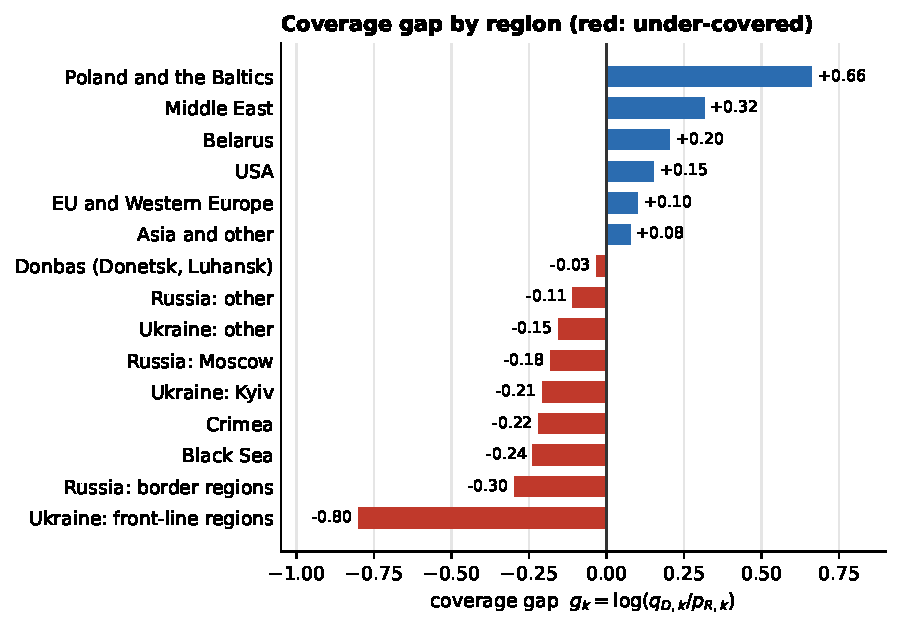
\includegraphics[width=0.62\textwidth]{figures/fig_geo_gap.pdf}
\caption{Coverage gap by region group: log ratio of each region's share of location mentions in my feed to its share in the basket. Red bars are under-covered, blue bars over-covered. The largest gap is for the Ukrainian front-line regions ($-0.80$, less than half the basket's share), followed by Russian border regions, the Black Sea and Crimea; the largest positive gap is for Poland and the Baltic states ($+0.66$, almost double).}
\label{fig:geogap}
\end{figure}

\begin{figure}[H]
\centering
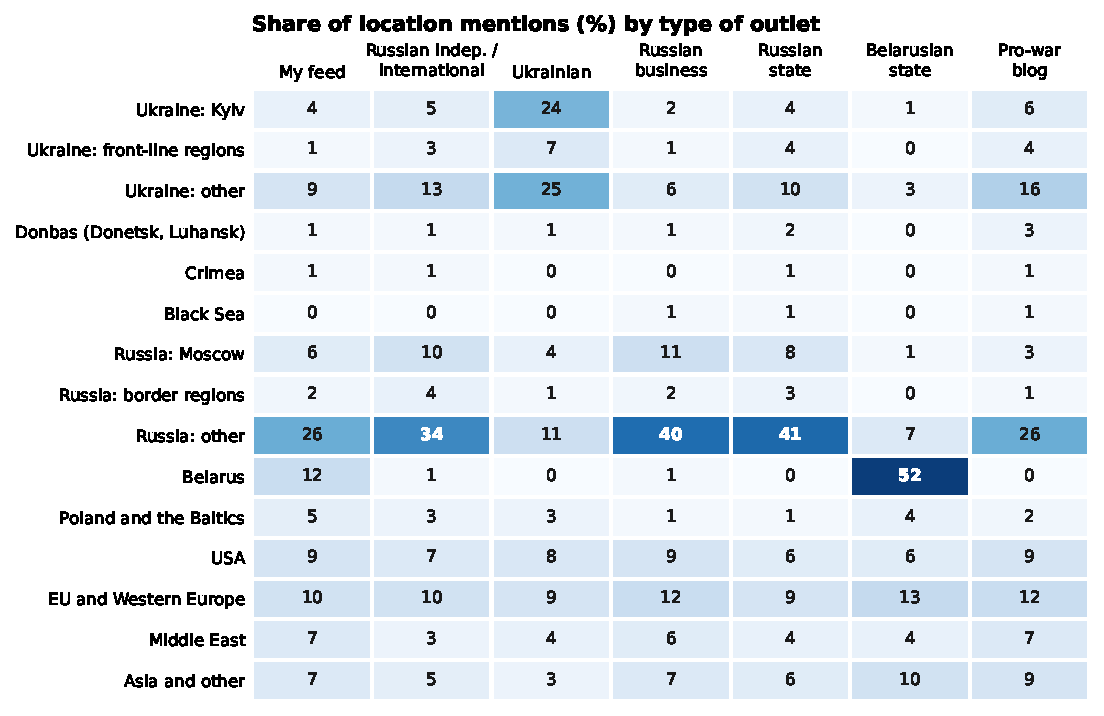
\includegraphics[width=0.86\textwidth]{figures/fig_geo_heatmap.pdf}
\caption{Share of location mentions (\%) in each region group, by type of outlet; each column sums to 100, and darker cells mean a larger share. Each type of outlet concentrates on its own country: Ukrainian outlets on Kyiv and the rest of Ukraine (49\% together), Belarusian state media on Belarus (52\%), and Russian state and business media on Russia outside Moscow (41\% and 40\%). My feed is one of the most evenly spread columns. Its share for Belarus (12\%) is higher than in any other type of outlet except Belarusian state media, and its share for Poland and the Baltic states (5\%) is the highest of all.}
\label{fig:geoheat}
\end{figure}

\subsection{Codebook labels: does the result depend on the topic model?}
\label{sec:res-codebook}
\paragraph{Agreement} My labels and the LLM's agree on the 200 shared posts with $\kappa=0.90$, which is ``almost perfect'' on the usual scale, so the LLM's 400 labels were used for training. The two annotators were not fully independent, because both applied the same written rules. The value of $\kappa$ therefore shows that the codebook can be applied consistently, not that two readers working without shared rules would agree this closely.

\begin{table}[H]
\centering
\small
\caption{Codebook classifier, five-fold cross-validation.}
\label{tab:codebook-res}
\begin{tabular}{lccccc}
\toprule
Training labels & Posts & Classes & Accuracy & Macro-F1 & ARI with NMF topics \\
\midrule
Mine & 200 & 12 & 0.520 & 0.409 & 0.10 \\
LLM (used) & 400 & 13 & 0.593 & 0.464 & 0.12 \\
\bottomrule
\end{tabular}
\end{table}

\paragraph{Classifier} With 13 classes, chance accuracy is below 0.10, so an accuracy of 0.59 shows that the categories can be learned from the words of a post, and doubling the training set raised macro-F1 from 0.41 to 0.46. Performance per category depends on the number of examples and on how formulaic the posts are. Strikes are the easiest category (F1 0.77), because strike reports follow a fixed pattern; diplomacy and international politics reach 0.68 and 0.64. Categories with a dozen examples or fewer are hardly learned: Russian repression has a precision of 1.00 but a recall of 0.09 (11 posts), culture has an F1 of 0.11, and ``Other'', which by definition has no shared vocabulary, 0.15. Belarusian repression had only four examples in the LLM labels and was merged into ``Other''.

\paragraph{Codebook categories and topics} The adjusted Rand index between the two partitions is only 0.12. Figure~\ref{fig:codebook} shows where they agree and where they differ. Several categories correspond to a single topic: Russian repression to T7, courts (73\%); Belarus's state agenda to T12 (71\%); Russian politics to T2, the Duma elections (45\%); Ukrainian domestic politics to T17 (41\%). ``Strikes and casualties'', in contrast, is spread over five topics (T1, T3, T9, T13, T16). The topic model separates strike reports by \emph{source and format}: Ministry of Defence bulletins, local reports from Kyiv, air-defence tallies, the port of Odesa. The codebook groups them by \emph{type of event}. This agrees with the framing results: outlets describe the same events in vocabularies different enough to form separate topics. The comparison also shows a weakness of the topic model: T14 is a general topic that receives between a quarter and a half of the posts in Belarus society, economy, culture and ``Other''.

\begin{figure}[H]
\centering
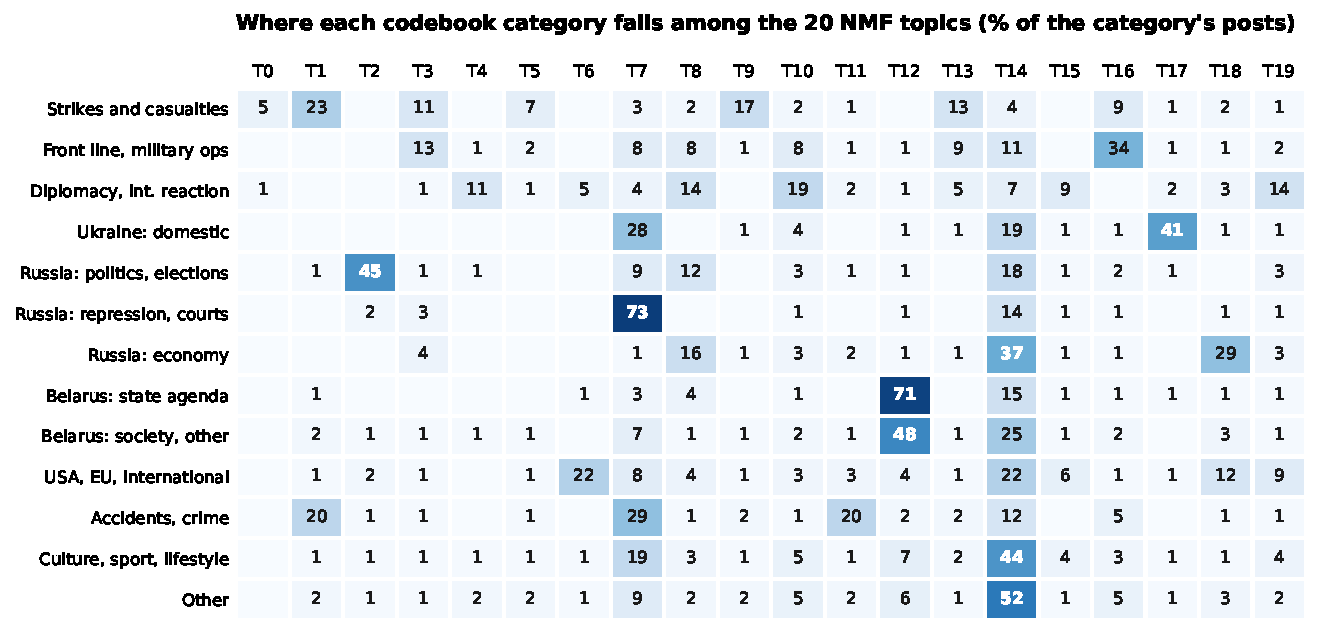
\includegraphics[width=\textwidth]{figures/fig_codebook_topics.pdf}
\caption{Share of each codebook category's posts (classifier labels on the full corpus) that the NMF model assigns to each topic. Rows sum to 100; darker cells mean a larger share, and values below 1 are left blank. A row with one dark cell, such as Russian repression (73\% in T7) or Belarus state agenda (71\% in T12), is a category that the topic model also finds as one topic. A row spread over several cells, such as strikes and casualties, is a category that the topic model divides further. The dark column T14 is the topic model's general catch-all topic.}
\label{fig:codebook}
\end{figure}

\paragraph{Echo score with hand-defined categories} Recomputed over codebook categories, my feed's echo score is 0.0148, and the equal-weight feed is narrower than only 9\% of all four-channel feeds (4\% when the classifier is trained on my own 200 labels). The absolute value cannot be compared with the topic score, because 13 discrete categories and 20 continuous topic shares give divergences on different scales, but the percentile can: under both category systems my feed is among the broadest tenth of possible feeds. The main result does not depend on the topic model.

\subsection{Framing: how the same strikes are described}
\label{sec:res-framing}
\paragraph{Distinctive vocabulary} Within the six strike-related topics (6,286 posts), state media (Russian and Belarusian) and the independent, international and Ukrainian outlets use clearly different vocabularies (Table~\ref{tab:fw}). State media describe the armed forces as having \ru{поразили}{hit} military targets such as logistics centres and cargo ships. Independent outlets describe Russian drones that \ru{атаковали}{attacked} Kyiv and damaged buildings and homes. Comparing my feed with the whole basket mostly finds Belarus-related words, for example \ru{Минск}{Minsk} with $z=16.2$, «беларусский» (Belarusian, opposition spelling), \ru{политзаключенный}{political prisoner}, \ru{Польша}{Poland} and \ru{Литва}{Lithuania}, because two of my four channels are Belarusian.

\begin{table}[H]
\centering
\small
\caption{Most distinctive words in strike reports, state vs.\ independent media (Fightin' Words $z$-scores; words are lemmas). A positive $z$ means the word is used more by state media, a negative $z$ more by independent media; $|z|>1.96$ is significant at about the 5\% level, so all words shown are strongly distinctive.}
\label{tab:fw}
\begin{tabular}{lr@{\hspace{2.5em}}lr}
\toprule
Distinctive of state media & $z$ & Distinctive of independent media & $z$ \\
\midrule
рф (RF, Russian Federation) & 35.9 & дрон (drone) & $-13.6$ \\
сообщить (to report) & 27.5 & удар (strike) & $-12.9$ \\
всу (Armed Forces of Ukraine) & 24.9 & российский (Russian) & $-12.0$ \\
поразить (to hit a target) & 24.1 & атаковать (to attack) & $-11.3$ \\
вс рф (Russian Armed Forces) & 23.1 & киев (Kyiv) & $-9.5$ \\
минобороны (Ministry of Defence) & 17.3 & беспилотник (unmanned drone) & $-9.3$ \\
логистический центр (logistics centre) & 14.1 & повредить (to damage) & $-6.7$ \\
сухогруз (cargo ship) & 12.2 & здание, дом (building, house) & $-6.7$, $-6.2$ \\
\bottomrule
\end{tabular}
\end{table}

\paragraph{Marker words} Figure~\ref{fig:markers} shows naming, sourcing and distancing words by type of outlet. «Беларусский» (the opposition spelling of ``Belarusian'') appears almost only in my feed (4.8 per 10,000 words), while «белорусский» (the official spelling) dominates Belarusian state media (41.5). \ru{ВСУ}{Armed Forces of Ukraine} is most frequent in Russian state media (38.6), and \ru{киевский режим}{``Kyiv regime''} in the pro-war blog (5.3). \ru{Война}{war} is most frequent in Ukrainian (28.7) and independent outlets (21.2), and \ru{СВО}{``special military operation''} in Russian state media and the pro-war blog. Ukrainian outlets that write in Russian use «ВСУ» and never «ЗСУ», the Ukrainian-language abbreviation.

\begin{figure}[H]
\centering
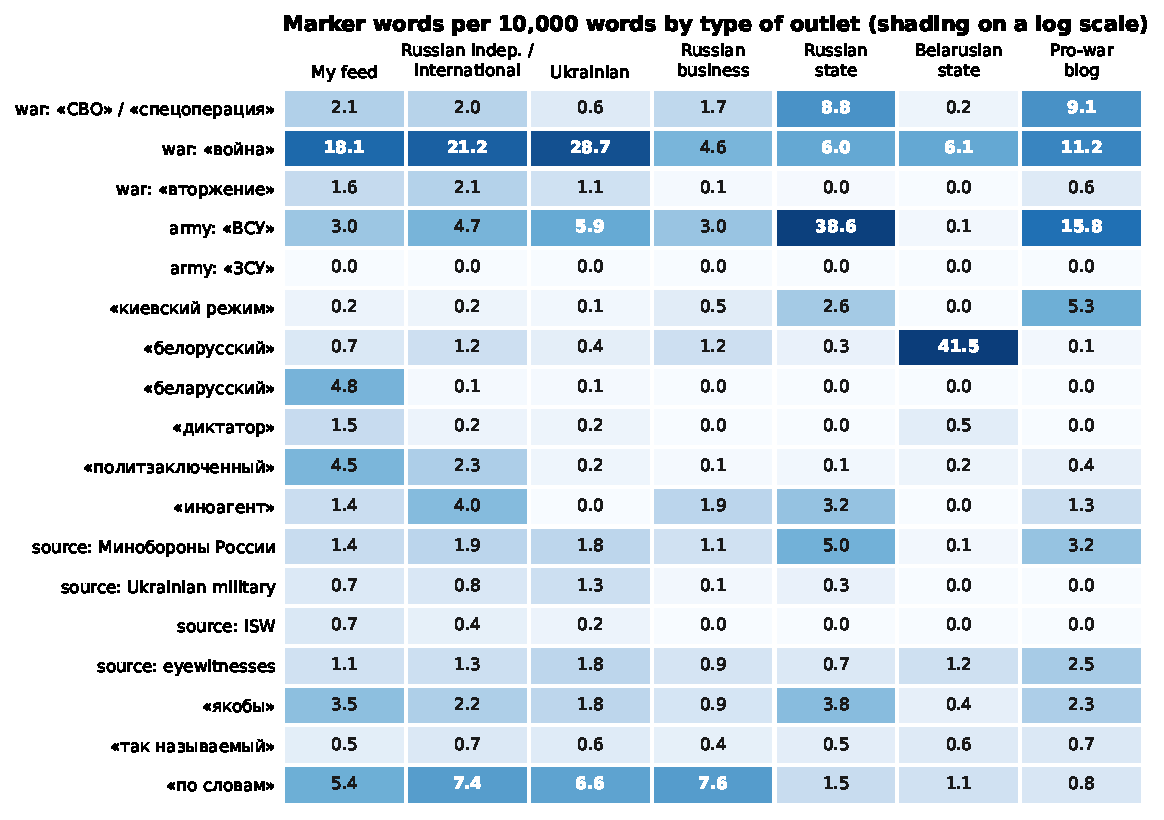
\includegraphics[width=0.9\textwidth]{figures/fig_markers.pdf}
\caption{Marker words per 10,000 words by type of outlet. Translations of the row labels: «СВО» / «спецоперация» ``special military operation''; «война» war; «вторжение» invasion; «ВСУ» / «ЗСУ» Armed Forces of Ukraine (Russian / Ukrainian abbreviation); «киевский режим» ``Kyiv regime''; «белорусский» / «беларусский» Belarusian (official / opposition spelling); «диктатор» dictator; «политзаключенный» political prisoner; «иноагент» ``foreign agent''; «Минобороны России» Russian Ministry of Defence; «якобы» allegedly; «так называемый» so-called; «по словам» according to. Shading is on a log scale so that both rare and frequent markers are visible; the numbers are the raw rates. Reading across a row compares outlets: the naming of the war, the army and Belarus separates the columns most clearly, while «по словам» and «якобы» are used by most outlets at similar rates.}
\label{fig:markers}
\end{figure}

\paragraph{Who is named as the attacker} The attacker rule was accurate on the hand-checked sample: 28 of 28 matches that could be judged were correct for the Russian side (precision 1.0; two matches could not be judged from the text) and 27 of 30 for the Ukrainian side (0.9). Table~\ref{tab:actors} and Figure~\ref{fig:actors} show the results.

\begin{table}[H]
\centering
\small
\caption{Share of strike posts (\%) that name each side as the attacker or use phrasing without an attacker: «в результате удара/атаки» (``as a result of a strike/attack'') and «прилёт» (literally ``an arrival'', meaning a hit).}
\label{tab:actors}
\begin{tabular}{lccccr}
\toprule
 & Russia & Ukraine & ``As a result & «прилёт» & Strike \\
 & named & named & of a strike'' & (no attacker) & posts \\
\midrule
My feed & 23.1 & 8.1 & 5.9 & 2.5 & 938 \\
Russian independent / international & 39.6 & 24.8 & 24.6 & 1.8 & 1,159 \\
Ukrainian & 12.7 & 3.3 & 4.6 & 20.4 & 1,766 \\
Russian business & 3.4 & 12.3 & 9.7 & 0.0 & 349 \\
Russian state & 5.0 & 13.1 & 3.7 & 0.1 & 1,708 \\
Belarusian state & 0.0 & 0.4 & 0.0 & 0.7 & 282 \\
Pro-war blog & 25.0 & 16.7 & 2.4 & 22.6 & 84 \\
\bottomrule
\end{tabular}
\end{table}

\begin{figure}[H]
\centering
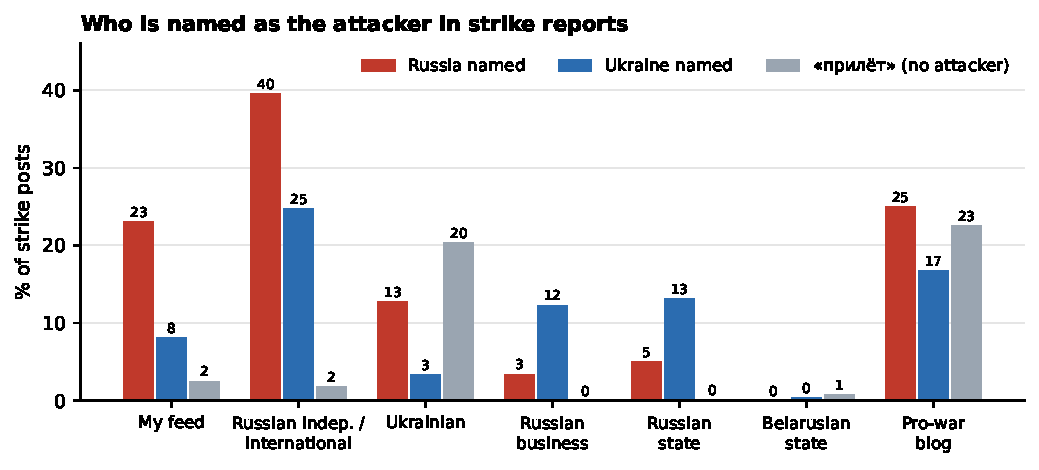
\includegraphics[width=0.85\textwidth]{figures/fig_actors.pdf}
\caption{Share of strike posts naming Russia (red) or Ukraine (blue) as the attacker, or using «прилёт» (``a hit'', grey), which leaves the attacker unstated. My feed and the independent outlets name Russia more often than Ukraine; Russian state and business media name Ukraine more often; Ukrainian outlets and the pro-war blog most often use «прилёт».}
\label{fig:actors}
\end{figure}

My feed names Russia as the attacker almost three times as often as Ukraine (23\% compared with 8\%). Russian state and business media reverse the ratio (5\% compared with 13\%, and 3\% compared with 12\%). They name Ukraine when its drones hit Russian regions, but describe Russia's own strikes with targets that were \ru{поражены}{hit}, a passive form without a grammatical subject, which the rule does not count. The independent and international outlets name both sides most often. Ukrainian outlets rarely name either side and write «прилёт» instead (20\%); in Ukrainian news the attacker is understood from context. Belarusian state media almost never describe strikes in these terms. These shares are lower bounds, because the rule finds an attacker only when it appears next to an attack word.

% ------------------------------------------------------------------ 6
\section{Interactive dashboard}
\label{sec:selector}
The analysis is also available as an interactive web dashboard (\todo{Vercel link}), kept in a separate repository from the pipeline. The notebook exports the channel profiles (topic mixes $\theta_s$, region shares and topic labels) to a small JSON file, and the dashboard recomputes everything else in the browser. A reader selects any combination of the 19 channels, optionally adjusts reading weights, and the dashboard shows:
\begin{itemize}
\item the topic and geographic echo scores of that feed;
\item its percentile among all feeds with the same number of channels, computed exactly over every combination, with a histogram of that distribution;
\item the coverage gap for every topic and every region group, as in Figures~\ref{fig:topicgap} and~\ref{fig:geogap}.
\end{itemize}
Presets select my feed, all channels, or one type of outlet. Because the null model is recomputed for each selection, the dashboard applies the same method to any feed, not only mine: anyone who reads some of these channels can see which subjects and places their combination covers less than the basket. The same selector is also included in the notebook as a Colab widget.

% ------------------------------------------------------------------ 7
\section{Discussion}
\label{sec:discussion}

\subsection{Results compared with expectations}
I expected my feed to be an echo chamber. By topic, the result is the opposite: four channels that seem similar to me (exile, independent, Belarus-focused) together cover the month's subjects in nearly the same proportions as 19 channels from across the spectrum. The convexity argument in Section~\ref{sec:results} explains this: each channel is unusual, but in a different direction. The remaining differences are real but specific. My feed under-covers the war's routine bulletins (the Ministry of Defence's daily claims, air-defence tallies and local strike reports) and the places they describe: the front-line regions, Russian border regions and Crimea. It over-covers Belarus, Poland and Lithuania, where the Belarusian opposition is based in exile. Geography separates my feed from the basket more than topics do (echo 0.0098 compared with 0.0038), and the classifier's blind-spot rates and the topic gaps agree on which topics are missing.

The classifier results explain why the topic difference is small although my feed seems distinctive to me. The classifier recognises my feed's posts within the corpus but performs at chance on unseen channels, and a classifier given only topic mixes performs worse still. What my channels have in common is wording rather than agenda: «беларусский» (the opposition spelling of ``Belarusian''), \ru{диктатор}{dictator}, \ru{политзаключенный}{political prisoner}, and \ru{война}{war} rather than \ru{СВО}{``special military operation''}. The framing analysis shows the same pattern across the whole basket: state and independent media cover the same strikes, but state media write about targets that were «поражены» (hit) at logistics centres, and independent media about drones that hit homes. Comparing sources directly, rather than starting from political labels, made these differences visible; a left/right label would not have captured them.

The project also shows why stability checks are necessary. My first topic model (LDA, $K=8$) suggested that my feed under-covers Belarus's official agenda. This finding disappeared once I used stable topics, because LDA's topics changed with the random seed.

\subsection{What ``echo chamber'' means here}
The echo score measures distance from the basket average. It does not measure quality or accuracy. The basket includes Russian and Belarusian state channels and a pro-war blog, so a feed close to the average has partly adopted their agenda. A low score is therefore not automatically good, and a high score is not automatically bad. In the Russian-language news space, the usual idea of an echo chamber is partly reversed: many readers, including me, choose their feed deliberately to avoid state propaganda, and part of the distance between my feed and the basket reflects that choice rather than a blind spot. The question this project can answer is narrower: which subjects, places and actors the sources I left out cover and my feed does not. This allows me to judge, topic by topic, whether I am missing information or only a framing I chose to avoid.

\subsection{Access to reliable information}
Since 2022, Russia has blocked most independent media and designated many journalists and outlets as ``foreign agents''. In Belarus, independent outlets, including two of the four channels in my feed, have been designated ``extremist'' since 2020--2021. The remaining independent outlets operate from exile, and Telegram is one of the main sources of news for Russian-speaking readers, alongside state and pro-war channels that publish at much higher volume (Figure~\ref{fig:volume}). Readers have to choose sources without being able to verify most claims themselves. For this reason it is useful to measure what even a carefully chosen feed leaves out.

\subsection{Limits of the method: propaganda and reporting}
Every model in this project works on word counts. A state post and an independent post about the same strike fall into the same topic, and a false claim written in neutral language looks the same as a true one. Separating them would require checking individual claims against outside evidence, which a word-frequency model cannot do. The framing measures in Section~\ref{sec:res-framing} are a first step in that direction. They make specific techniques measurable: naming or omitting the attacker (state media name Ukraine as the attacker more often than Russia, and describe Russia's own strikes with the passive «поражены», ``were hit''), loaded labels (\ru{киевский режим}{``Kyiv regime''}, and «СВО» rather than «война»), and reliance on official sources (\ru{сообщили в Минобороны}{the Ministry of Defence reported}). These are indicators, not judgements of accuracy. A next step would be to extract specific claims, such as casualty figures or claimed targets, and compare them across outlets and with independently verified reports.

\subsection{Ethics of the data}
All posts come from the public web previews of public channels. No private messages, user accounts or reader data were collected. The crawler waited 1.5--3 seconds between requests and identified itself as a research crawler. All quoted posts come from outlets, not private individuals. State and pro-war channels are analysed as data on how events are presented and are not used as sources of fact.

\subsection{Limitations}
\begin{itemize}
\item \textbf{Time window.} Five weeks of news include one-off stories (the Flydubai incident appears as an over-covered ``topic'') and the Russian parliamentary elections.
\item \textbf{Basket composition.} The basket is my choice. The Belarusian state channels affect the echo score most, and the Ukrainian side has no state or public broadcaster in the basket, because those publish in Ukrainian.
\item \textbf{Reading weights.} The weights are my own estimate, not measured from my Telegram activity. Section~\ref{sec:weights} shows that the topic result holds for balanced reading but not if one channel, especially Zerkalo, dominates.
\item \textbf{Place mapping.} The mapping from place names to region groups covers 74\% of location mentions; the rest are mostly small towns, districts and countries outside the main groups.
\item \textbf{Word-pattern rules.} The marker words and the attacker rule are word patterns. The attacker rule was checked by hand on 60 matches (precision 0.9--1.0), but it misses attackers that are not next to an attack word, so its shares are lower bounds; its recall was not measured.
\item \textbf{Codebook annotators.} The second annotator was an LLM working in a chat session from the same written rules. This is less reproducible than a scripted API call at temperature 0, and the two annotators were not fully independent. The labels are saved as a file so that the analysis can be rerun.
\item \textbf{Lemmatisation errors.} pymorphy3 assigns lemmas by matching a word against a dictionary of Russian inflection patterns, and guesses from the word's ending when the word is not in the dictionary. Abbreviations, transliterated foreign names and new military terms do not follow these patterns. For example, \ru{БПЛА}{UAV, an abbreviation of ``unmanned aerial vehicle''} is not inflected like a regular noun, so pymorphy3 analyses it as a form of a non-existent verb, «бпнуть». Such errors split or mislabel some features, although they affect all outlets in the same way. Separately, topic T1 combines strike casualties with road accidents, because both are reported with similar words (``killed'', ``injured'', ``hospitalised'').
\end{itemize}

\subsection{Next steps}
\begin{itemize}
\item \textbf{More codebook labels.} Label more posts in the small categories (repression, culture) and add a second human annotator, so that agreement is measured between independent readers.
\item \textbf{Framing from syntax.} Replace word patterns with dependency parsing, so that the attacker is identified from sentence structure rather than word distance.
\item \textbf{Translation.} Add Ukrainian-language state and public media in translation, after testing whether translation leaves detectable traces in the text.
\item \textbf{Longer time window.} Extend the corpus beyond five weeks so that single events carry less weight.
\end{itemize}

% ------------------------------------------------------------------ 8
\section{Conclusion}
\begin{enumerate}
\item \textbf{My feed is broad by topic.} Its echo score is lower than that of 98.2\% of all possible four-channel feeds, because its channels deviate from the basket in different directions and largely cancel out. Categories I defined myself give the same result (the broadest 4--9\% of feeds). This holds when I read my channels in similar proportions; a feed dominated by one channel would be narrow.
\item \textbf{The gaps are specific.} My feed under-covers routine military bulletins (front-line claims, air-defence tallies, local strike reports) and the places they describe; two independent methods identify the same topics.
\item \textbf{My channels share wording, not agenda.} Classifiers recognise my feed within the corpus (ROC-AUC up to 0.90) but not on unseen channels (0.50), and topic features alone carry almost no signal.
\item \textbf{Framing differs more than coverage.} Outlets describe the same strikes in different vocabularies and differ clearly in whether they name an attacker.
\item \textbf{Methodological checks changed the conclusions.} Selecting the topic model by stability removed a finding that came from LDA's random seed, and removing channel signatures eliminated a large source of leakage from the classifier.
\end{enumerate}

% ------------------------------------------------------------------ AI
\section*{AI statement}
\addcontentsline{toc}{section}{AI statement}
\todo{Check and edit this statement so that it matches what you did.} I used Claude (Anthropic) as a programming and writing assistant: to draft and debug parts of the notebook code (the crawler, caching to Google Drive, topic-model selection and plotting) and the dashboard, to suggest additional methods and checks, to act as the second annotator for the codebook labels (Section~\ref{sec:res-codebook}), and to help edit and typeset this report in \LaTeX. I chose the research question, the channels in my feed and in the reference basket, and the reading weights; ran the data collection and every analysis in Colab; read and labelled the topics; checked the attacker rule by hand; labelled 200 posts against the codebook; and interpreted the results.

% ------------------------------------------------------------------ refs
\section*{References}
\addcontentsline{toc}{section}{References}
\begin{small}
\begin{itemize}[leftmargin=1.2em,label={}]
\setlength{\itemindent}{-1.2em}
\item Blei, D. M., Ng, A. Y., \& Jordan, M. I. (2003). Latent Dirichlet allocation. \emph{Journal of Machine Learning Research}, 3, 993--1022.
\item Bouma, G. (2009). Normalized (pointwise) mutual information in collocation extraction. \emph{Proceedings of GSCL}, 31--40.
\item Hubert, L., \& Arabie, P. (1985). Comparing partitions. \emph{Journal of Classification}, 2, 193--218.
\item Korobov, M. (2015). Morphological analyzer and generator for Russian and Ukrainian languages. \emph{AIST 2015}. Used through pymorphy3.
\item Lee, D. D., \& Seung, H. S. (1999). Learning the parts of objects by non-negative matrix factorization. \emph{Nature}, 401, 788--791.
\item Lin, J. (1991). Divergence measures based on the Shannon entropy. \emph{IEEE Transactions on Information Theory}, 37(1), 145--151.
\item Monroe, B. L., Colaresi, M. P., \& Quinn, K. M. (2008). Fightin' words: Lexical feature selection and evaluation for identifying the content of political conflict. \emph{Political Analysis}, 16(4), 372--403.
\item Natasha project. Natasha (named-entity recognition) and razdel (tokenisation) for Russian. \url{https://github.com/natasha}.
\item Pedregosa, F., et al. (2011). Scikit-learn: Machine learning in Python. \emph{Journal of Machine Learning Research}, 12, 2825--2830.
\item Platt, J. (1999). Probabilistic outputs for support vector machines and comparisons to regularized likelihood methods. \emph{Advances in Large Margin Classifiers}, 61--74.
\item Rennie, J. D., Shih, L., Teevan, J., \& Karger, D. R. (2003). Tackling the poor assumptions of naive Bayes text classifiers. \emph{ICML 2003}, 616--623.
\item Röder, M., Both, A., \& Hinneburg, A. (2015). Exploring the space of topic coherence measures. \emph{WSDM 2015}, 399--408.
\item Schofield, A., Magnusson, M., \& Mimno, D. (2017). Pulling out the stops: Rethinking stopword removal for topic models. \emph{EACL 2017}, 432--436.
\item Wang, S., \& Manning, C. D. (2012). Baselines and bigrams: Simple, good sentiment and topic classification. \emph{ACL 2012}, 90--94.
\item Telegram channel web previews, \texttt{https://t.me/s/<handle>}, used as the data source (collected 8 and 13 October 2026).
\end{itemize}
\end{small}

% ------------------------------------------------------------------ appendix
\appendix
\section{Code excerpts: methods implemented from scratch}
\label{app:code}
The full pipeline is in the notebook. The metrics below are not available in standard libraries and were implemented directly from their definitions.

\subsection*{A.1 Jensen--Shannon divergence and the exhaustive null model}
\vspace{4pt}
\begin{lstlisting}
def jsd(q, p, eps=1e-12):
    """Jensen-Shannon divergence in base 2; works row-wise on 2-D arrays."""
    # small constant so that log(0) never occurs, then renormalise to probability vectors
    q, p = np.asarray(q) + eps, np.asarray(p) + eps
    q, p = q / q.sum(-1, keepdims=True), p / p.sum(-1, keepdims=True)
    m = 0.5 * (q + p)                                  # mixture distribution
    kl = lambda a, b: (a * np.log2(a / b)).sum(-1)     # KL divergence in bits
    return 0.5 * kl(q, m) + 0.5 * kl(p, m)

Theta = theta_s.to_numpy()                 # channel x topic profiles (19 x 20)
null = {}
for k in range(1, n_ch + 1):               # every feed size from 1 to 19 channels
    # all combinations of k channels; each feed is the equal-weight mean of its channels
    combos = np.array(list(combinations(range(n_ch), k)))
    null[k] = jsd(Theta[combos].mean(axis=1), p_R[None, :])

# percentile: share of four-channel feeds that are closer to the basket than my feed
diet_equal = jsd(theta_s.loc[DIET].mean(axis=0).to_numpy(), p_R)
pct = (null[4] < diet_equal).mean() * 100
\end{lstlisting}

\subsection*{A.2 NPMI topic coherence}
\vspace{4pt}
\begin{lstlisting}
def npmi_coherence(components, Xb, top_n=10):
    """Mean NPMI over pairs of each topic's top words, from post-level co-occurrence.

    components: topic-word weights (one row per topic); Xb: binary post-word matrix.
    """
    n, scores = Xb.shape[0], []
    for comp in components:
        top = np.argsort(comp)[::-1][:top_n]            # the topic's top words
        sub = Xb[:, top]
        co = (sub.T @ sub).toarray() / n                # P(w_i, w_j); the diagonal is P(w_i)
        p = np.diag(co).copy()
        vals = []
        for i in range(top_n):
            for j in range(i + 1, top_n):
                pij = co[i, j]
                # NPMI is -1 by definition for a pair that never occurs together
                vals.append(-1.0 if pij == 0 else np.log(pij / (p[i] * p[j])) / -np.log(pij))
        scores.append(np.mean(vals))                    # coherence of one topic
    return np.array(scores)
\end{lstlisting}

\subsection*{A.3 Fightin' Words (log-odds with an informative Dirichlet prior)}
\vspace{4pt}
\begin{lstlisting}
def fightin_words(texts_a, texts_b, background, alpha0=500, min_df=10):
    """z-scores of the log-odds ratio of each word between groups A and B (Monroe et al., 2008)."""
    # word and two-word counts in group A, group B and the whole background corpus
    vec = CountVectorizer(ngram_range=(1, 2), min_df=min_df).fit(background)
    ya = np.asarray(vec.transform(texts_a).sum(axis=0)).ravel()
    yb = np.asarray(vec.transform(texts_b).sum(axis=0)).ravel()
    bg = np.asarray(vec.transform(background).sum(axis=0)).ravel()
    # prior pseudo-counts proportional to each word's background frequency, alpha0 in total
    alpha = bg / bg.sum() * alpha0
    na, nb = ya.sum(), yb.sum()
    # difference in smoothed log-odds between the two groups
    delta = (np.log((ya + alpha) / (na + alpha0 - ya - alpha))
             - np.log((yb + alpha) / (nb + alpha0 - yb - alpha)))
    # divide by the approximate standard error (delta method: Var[log y] ~ 1/y)
    z = delta / np.sqrt(1 / (ya + alpha) + 1 / (yb + alpha))
    return pd.Series(z, index=vec.get_feature_names_out())
\end{lstlisting}

\end{document}
